% !TeX spellcheck = hu_HU
% !TeX encoding = UTF-8
% !TeX program = xelatex
% TODO Change language to en_GB (recommended) or en_US for English documents
\documentclass[11pt,a4paper,oneside]{report}             % Single-side
%\documentclass[11pt,a4paper,twoside,openright]{report}  % Duplex

% thanks to http://tex.stackexchange.com/a/47579/71109
\usepackage{ifxetex}
\usepackage{ifluatex}
\newif\ifxetexorluatex % a new conditional starts as false
\ifnum 0\ifxetex 1\fi\ifluatex 1\fi>0
   \xetexorluatextrue
\fi

\ifxetexorluatex
  \usepackage{fontspec}
\else
  \usepackage[T1]{fontenc}
  \usepackage[utf8]{inputenc}
  \usepackage[lighttt]{lmodern}
  \ttfamily\DeclareFontShape{T1}{lmtt}{m}{it}{<->sub*lmtt/m/sl}{}
\fi

\usepackage[english,magyar]{babel} % Alapértelmezés szerint utoljára definiált nyelv lesz aktív, de később külön beállítjuk az aktív nyelvet.

\usepackage{emptypage} % omit page number on empty pages

%\usepackage{cmap}
\usepackage{amsfonts,amsmath,amssymb} % Mathematical symbols.
%\usepackage[ruled,boxed,resetcount,linesnumbered]{algorithm2e} % For pseudocodes. % beware: this is not compatible with LuaLaTeX, see http://tex.stackexchange.com/questions/34814/lualatex-and-algorithm2e
\usepackage{booktabs} % For publication quality tables for LaTeX
\usepackage{graphicx}

%\usepackage{fancyhdr}
%\usepackage{lastpage}

\usepackage{anysize}
%\usepackage{sectsty}
\usepackage{setspace} % For setting line spacing

\usepackage[unicode]{hyperref} % For hyperlinks in the generated document.
\usepackage{xcolor}
\usepackage{listings} % For source code snippets.

\usepackage[amsmath,thmmarks]{ntheorem} % Theorem-like environments.

\usepackage[hang]{caption}

\usepackage{subfigure}

\singlespacing

\newcommand{\selecthungarian}{
	\selectlanguage{magyar}
	\setlength{\parindent}{2em}
	\setlength{\parskip}{0em}
	\frenchspacing
}

\newcommand{\selectenglish}{
	\selectlanguage{english}
	\setlength{\parindent}{0em}
	\setlength{\parskip}{0.5em}
	\nonfrenchspacing
	\renewcommand{\figureautorefname}{Figure}
	\renewcommand{\tableautorefname}{Table}
	\renewcommand{\partautorefname}{Part}
	\renewcommand{\chapterautorefname}{Chapter}
	\renewcommand{\sectionautorefname}{Section}
	\renewcommand{\subsectionautorefname}{Section}
	\renewcommand{\subsubsectionautorefname}{Section}
}

\usepackage[numbers]{natbib}
\usepackage{xspace}


%TODO Set the main variables
\newcommand{\vikszerzoVezeteknev}{Gáti}
\newcommand{\vikszerzoKeresztnev}{László Dávid}

\newcommand{\vikkonzulensAMegszolitas}{}
\newcommand{\vikkonzulensAVezeteknev}{Tóthné Farkas}
\newcommand{\vikkonzulensAKeresztnev}{Rebeka}

\newcommand{\vikkonzulensBMegszolitas}{}
\newcommand{\vikkonzulensBVezeteknev}{}
\newcommand{\vikkonzulensBKeresztnev}{}

\newcommand{\vikkonzulensCMegszolitas}{}
\newcommand{\vikkonzulensCVezeteknev}{}
\newcommand{\vikkonzulensCKeresztnev}{}

\newcommand{\vikcim}{Állapottérkép verifikációs MagicDraw plugin továbbfejlesztése} % Cím
\newcommand{\viktanszek}{\bmemit} % Tanszék
\newcommand{\vikdoktipus}{\msc} % Dokumentum típusa (\bsc vagy \msc)
\newcommand{\vikmunkatipusat}{diplomatervet} % a "hallgató nyilatkozat" részhez: szakdolgozatot vagy diplomatervet

\input{include/tdk-variables}
\newcommand{\szerzoMeta}{\vikszerzoVezeteknev{} \vikszerzoKeresztnev} % egy szerző esetén
%\newcommand{\szerzoMeta}{\vikszerzoVezeteknev{} \vikszerzoKeresztnev, \tdkszerzoB} % két szerző esetén

%TODO Language configuration -- choose one
% Beállítások magyar nyelvű dolgozathoz
%--------------------------------------------------------------------------------------
% Elnevezések
%--------------------------------------------------------------------------------------
\newcommand{\bme}{Budapesti Műszaki és Gazdaságtudományi Egyetem}
\newcommand{\vik}{Villamosmérnöki és Informatikai Kar}

\newcommand{\bmemit}{Méréstechnika és Információs Rendszerek Tanszék}

\newcommand{\keszitette}{Készítette}
\newcommand{\konzulens}{Konzulens}

\newcommand{\bsc}{Szakdolgozat}
\newcommand{\msc}{Diplomaterv}
\newcommand{\tdk}{TDK dolgozat}
\newcommand{\bsconlab}{BSc Önálló laboratórium}
\newcommand{\msconlabi}{MSc Önálló laboratórium 1.}
\newcommand{\msconlabii}{MSc Önálló laboratórium 2.}

\newcommand{\pelda}{Példa}
\newcommand{\definicio}{Definíció}
\newcommand{\tetel}{Tétel}

\newcommand{\bevezetes}{Bevezetés}
\newcommand{\koszonetnyilvanitas}{Köszönetnyilvánítás}
\newcommand{\fuggelek}{Függelék}
\newcommand{\uppaal}{UPPAAL}

% Opcionálisan átnevezhető címek
%\addto\captionsmagyar{%
%\renewcommand{\listfigurename}{Saját ábrajegyzék cím}
%\renewcommand{\listtablename}{Saját táblázatjegyzék cím}
%\renewcommand{\bibname}{Saját irodalomjegyzék név}
%}

\newcommand{\szerzo}{\vikszerzoVezeteknev{} \vikszerzoKeresztnev}
\newcommand{\vikkonzulensA}{\vikkonzulensAMegszolitas\vikkonzulensAVezeteknev{} \vikkonzulensAKeresztnev}
\newcommand{\vikkonzulensB}{\vikkonzulensBMegszolitas\vikkonzulensBVezeteknev{} \vikkonzulensBKeresztnev}
\newcommand{\vikkonzulensC}{\vikkonzulensCMegszolitas\vikkonzulensCVezeteknev{} \vikkonzulensCKeresztnev}

\newcommand{\selectthesislanguage}{\selecthungarian}

\bibliographystyle{huplain}

\def\lstlistingname{lista}

\newcommand{\appendixnumber}{6}  % a fofejezet-szamlalo az angol ABC 6. betuje (F) lesz

% Settings for English documents
%\input{include/thesis-en}

\input{include/preamble}

%--------------------------------------------------------------------------------------
% Table of contents and the main text
%--------------------------------------------------------------------------------------
\begin{document}

\pagenumbering{gobble}

%TODO These includes define guidelines -- remove these
%~~~~~~~~~~~~~~~~~~~~~~~~~~~~~~~~~~~~~~~~~~~~~~~~~~~~~~~~~~~~~~~~~~~~~~~~~~~~~~~~~~~~~~

%--------------------------------------------------------------------------------------
% Feladatkiiras (a tanszeken atveheto, kinyomtatott valtozat)
%--------------------------------------------------------------------------------------



\selectthesislanguage

%TODO Titlepage -- choose one from below
%~~~~~~~~~~~~~~~~~~~~~~~~~~~~~~~~~~~~~~~~~~~~~~~~~~~~~~~~~~~~~~~~~~~~~~~~~~~~~~~~~~~~~~
\include{include/titlepage}		   % Szakdolgozat/Diplomaterv címlap
%\include{include/titlepage-tdk}	% TDK címlap
%\include{include/titlepage-otdk}   % OTDK címlap


% Table of Contents
%~~~~~~~~~~~~~~~~~~~~~~~~~~~~~~~~~~~~~~~~~~~~~~~~~~~~~~~~~~~~~~~~~~~~~~~~~~~~~~~~~~~~~~
\tableofcontents\cleardoublepage


% Declaration and Abstract
%~~~~~~~~~~~~~~~~~~~~~~~~~~~~~~~~~~~~~~~~~~~~~~~~~~~~~~~~~~~~~~~~~~~~~~~~~~~~~~~~~~~~~~
\include{include/declaration} %TODO Hallgatói nyilatkozat -- TDK és OTDK esetén törlendő!
\pagenumbering{roman}
\setcounter{page}{1}

\selecthungarian

%----------------------------------------------------------------------------
% Abstract in Hungarian
%----------------------------------------------------------------------------
\chapter*{Kivonat}\addcontentsline{toc}{chapter}{Kivonat}


Biztonságkritikus rendszerek tervezéséhez különösen fontos, hogy rendelkezésünkre álljanak olyan eszközök, melyek segítségével meg lehet vizsgálni, hogy a rendszer modellezett viselkedése valóban megfelel a rendszerrel szemben támasztott követelményeknek. A viselkedés modellezése magas szinten gyakran történik állapot alapú formalizmusokkal, mint például a UML állapottérképekkel. Ezek gyakran komponenseket definiálnak amik egymással kölcsönhatásban állnak, így szükségessé válik ezeknek a komponens együtteseknek a vizsgálata is. A tulajdonságok teljesüléséhez példákat kell szolgáltatni amik alátámasztják a tulajdonság teljesülését vagy adott esetben sérülését, hogy a mérnökök megtalálhassák és kijavíthassák a tervezési hibákat.

A MagicDraw egy UML és SysML modellező eszköz amely elterjedt az iparban. Ehhez az eszközhöz korábbi munkáim során készítettem egy beépülő modult, ami lehetővé teszi logikai formulák segítségével specifikált tulajdonságok teljesülésének ellenőrzését állapottérképeken. A mérnökök gyakran használnak hierarchikus, komponens alapú állapot modelleket rendszerek modellezésére, azonban a beépülő modul ezek együttes ellenőrzésére nem képes. A tulajdonságok teljesülésének vizsgálata olyan példák keresését jelenti, amik bizonyítják ennek teljesülését. Fontos, hogy a mérnökök ezekhez hozzáférjenek és elemezni tudják. A beépülő modul ezeket megjelenítésére nem képes.

Dolgozatomban bemutatom a beépülő modult és hogy milyen módon fejlesztettem azt tovább, hogy lehetőséget biztosítson komponenst alapú hierarchikus állapot modellek formális ellenőrzésére és az ellenőrzés során keletkező bizonyítékként szolgáló példák megjelenítésére. Az elkészítette eszköz működését egy példán keresztül bemutatom, majd mérések segítségével értékelem a gyakorlati megvalósítás hatékonyságát.


\vfill
\selectenglish


%----------------------------------------------------------------------------
% Abstract in English
%----------------------------------------------------------------------------
\chapter*{Abstract}\addcontentsline{toc}{chapter}{Abstract}

Safety critical systems raise the need for various tools that can verify their design by checking if modeled behaviors satisfy their specified requirements.

Modeling behaviors on a high level often relies on state-based formalisms such as UML statecharts. These often serve as definitions for components that influence each other’s behavior through various types of communication. This makes it necessary that the tools support this kind of modeling and allow model checking on such component-based systems. The existence of required system properties must be proven by examples that either prove or disprove the existence of these specified properties. Engineers then can use these examples to find and correct errors in the model.

MagicDraw is a modeling tool for UML and SysML and it is a widely used tool amongst system engineers. In the course of my previous works, I have made a plugin for this modeling tool which enables the check of properties defined as logical formulas on statecharts. However, it cannot perform checks on models that follow the commonly used component-based approach. The existence of properties is proven by finding examples as proof of their existence. It is important that engineers can view and analyze these examples which the tool does not allow just yet.

In my thesis I introduce the tool that I have made previously and the feature improvements that allow the checking of component-based systems and the display of examples produced during the checking process. I present my solutions on a small-scale example then I perform some measurements to evaluate the performance of the used solutions.


\vfill
\cleardoublepage

\selectthesislanguage

\newcounter{romanPage}
\setcounter{romanPage}{\value{page}}
\stepcounter{romanPage}    %TODO Összefoglaló -- TDK és OTDK esetén nem kötelező


% The main part of the thesis
%~~~~~~~~~~~~~~~~~~~~~~~~~~~~~~~~~~~~~~~~~~~~~~~~~~~~~~~~~~~~~~~~~~~~~~~~~~~~~~~~~~~~~~
\pagenumbering{arabic}

%TODO import your own content
%----------------------------------------------------------------------------
\chapter{\bevezetes}
%----------------------------------------------------------------------------

A IT technológiák térnyerésével egyre több és komplexebb rendszer készül, melyeknek sokszor valós időben kell működni. Mivel ilyen rendszerek jellemzően valamilyen biztonság kritikus környezetben működnek, elengedhetetlené válik ezek gondos megtervezése és átfogó vizsgálata különösen a helyes működés tekintetében.

A tervezés és ellenőrzés költséges, időigényes folyamat, ezért szükség van olyan eszközökre amelyek megkönnyítik vagy akár teljesen automatizálnak egyes folyamatokat. A tervezés során általában valamilyen modellvezért technikát alkalmaznak, melynek középpontjában a modellek állnak. A tervezés során elkészített tervek nagyon sok értékes információt tartalmaznak, melyeket újra fel tudunk használni és származtatni ezekből kódot, dokumentációt, vagy akár más modelleket, ezáltal időt és erőforrásokat megtakarítva. Ráadásul mivel ezeket automatikusan gépek végzik, minimalizálódnak az emberi hibák például a programkódban, ahhoz képest mintha ezeket kézzel végeznénk el.

Terveinket már érdemes a tervezés korai fázisaiban ellenőrizni, hiszen az itt vétett hibák akár kritikusak lehetnek a későbbiekben. Az ellenőrzésekhez szintén fel tudjuk használni a modelljeinket és szimulálni tudjuk a rendszert, vagy képesek vagyunk magát a modellt is vizsgálni formális módszerek segítségével.

A MagicDraw egy mára de-facto ipari standarddá vált szoftver, és rendszer architektúra modellező eszköz ami fejlett grafikus interfészt nyújt a felhasználók számára. Modelleket elsősorban egy általános célú modellezési nyelvvel UML-el lehet készíteni, azonban UML profilok segítségével akár saját szakterület specifikus nyelvek használatára is lehetőségünk nyílik. Ilyen formában a MagicDraw lehetővé teszi modellek létrahozását SysML nyelven is amihez a profilt maga biztosítja. A dolgozat a továbbiakban SysML modellekkel foglalkozik.

Ugyan a MagicDraw számos fontos és hasznos funkcióval rendelkezik, még mindig megvan az igény újabbakra főleg Verifikáció/Validáció tekintetében. A MagicDrawToGamma nevű MagicDrawhoz készült plugin SysML állapottérképek formális verifikálásához nyújt megoldást, melyhez a Gamma Statechart Composition Frameworköt és az UPPAAL nevű eszközöket használja fel.

Az eszköz ugyan \emph{Proof of Concept} jelleggel már képes a verifikációt elvégezni, azonban, hogy akár szélesebb körben is használható eszközzé válhasson még sok tekintetben fejlesztésre szorul. Jelen dolgozat célja bemutatni azokat a fejlesztéseket amiket a mesterképzés során végeztem az eszközön és visszatekintve kiértékelni azokat a mérnöki megoldásokat melyeket a fejlesztés során hoztam.

A dolgozat felépítése a következő: a második fejezetben ismertetem azokat az ismereteket amelyek a dolgozat során felvetülő problémák illetve az ezekre adott megoldások megértéséhez szükségesek. A harmadik fejezetben ismertetem a projekt céljait és az ezekhez vezető utat, alkalmazott megoldásokat, illetve bemutatom a beépülő modul működését. A negyedik fejezetben pedig értékelem az alkalmazott megoldások hatékonyságát és az elkészített plugint.
\chapter{Háttérismeretek}

Ebben a fejezetben bemutatom azokat az ismereteket, technológiákat amelyek segítenek megérteni azokat a megoldásokat melyeket a dolgozat elkészítése során alkalmaztam.

\section{Kapocsolódó munkák}
A fejlesztés megkezdése előtt utána néztem, hogy milyen eszközök állak rendelkezésre, amelyek hasonló problémákat oldanak meg. Specifikusan a MagicDrawhoz nem találtam olyat, ami még most is releváns lenne (korábbi munkáim során találkoztam hasonló célú eszközzel, de úgy tűnik annak a fejlesztése nem folytatódott). Általánosabban az állapottérkép és formális verifikációval kapcsolatban a legszorosabban kapcsolódó munka a Gamma Statechart Compoition Framework amelyet későbbi fejezetekben mutatok be. A megoldások amiket alkalmaztam főleg ennek az eszköznek a segítségével történtek.

\section{SysML \cite{SysML}}

A System Modeling Language (SysML) egy általános célú architektúra modellező nyelv, melyet elsősorban rendszermérnökök használnak. A nyelvvel különböző komplex rendszereket tudunk leírni többféle megközelítésből mint magas szintű funkcionális modellek mind pedig az alacsonyabb akár fizikai modellekig.

A SysML-t mint ahogyan az UML-t is az Object Management Group (OMG) fejleszti, sőt az UML 2-nek egy dialógusa a nyelv, úgynevezett UML profil segítségével van definiálva. Az UML profil a nyelv specializálásának egy módja sztereotípiák (Stereotype), megkötések (Constraint) és címkézett értékek (Tagged Value) segítségével (\refstruc{fig:custom-profile}).

\begin{figure}[!ht]
	\centering
	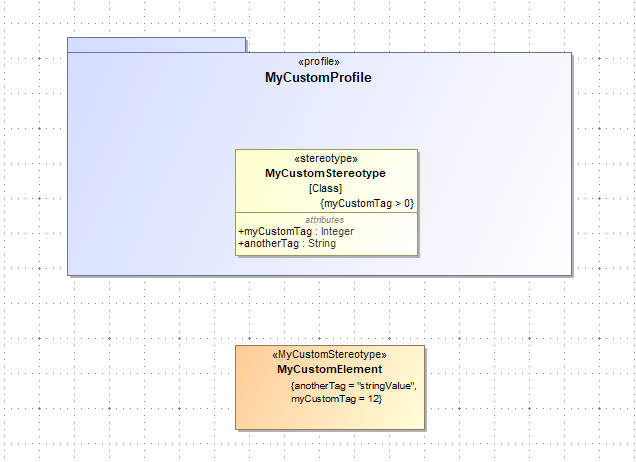
\includegraphics[width=150mm, keepaspectratio]{figures/preliminaries/custom-profile.png}
	\caption{UML nyelv specializálása sztereotípiákkal}
	\label{fig:custom-profile}
\end{figure}

Egy nyelv lehetséges elemeit és kapcsolatait leíró struktúrát metamodellnek hívjuk, a tényleges elemekből és ezek kapcsolatából álló modellt pedig példánymodellnek.  SysML esetében az UML profil az amit metamodellnek tudunk tekinteni, igaz a metaszintek eléggé összemosódnak és nem elegendő csak a profilt ismerni, hanem az UML metamodellt is ismerni kell. Például egy SysML Block valójában egy sztereotipizált UML Class. Ez azt jelenti, hogy van egy UML példány specifikáció (Instance Specification) aminek az osztálya (Classifier) egy Block sztereotípia és ez hozzá van rendelve az UML-s osztály példányunkhoz a modellünkben. Az UML-s osztály példány a sztereotípia és a példány specifikáció tehát hagyományos értelemben azonos metaszinten helyezkednek el (\refstruc{fig:block-stereotype}).

\begin{figure}[!ht]
	\centering
	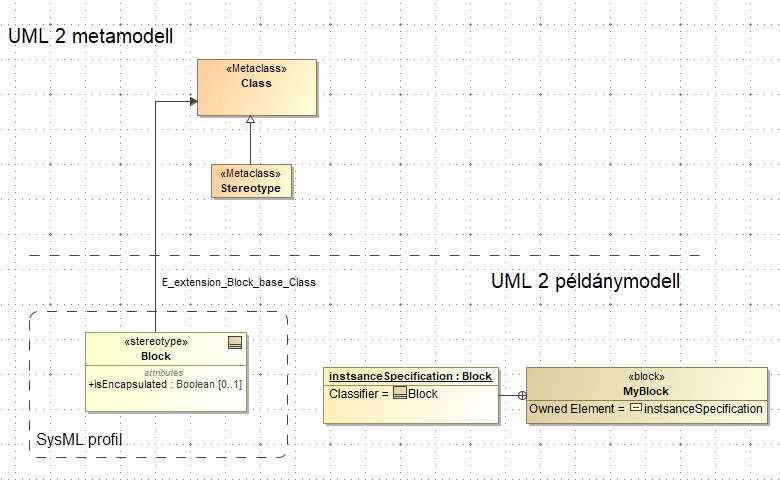
\includegraphics[width=150mm, keepaspectratio]{figures/preliminaries/block-stereotype.png}
	\caption{Meta szintek és Block sztereotípia alkalmazása}
	\label{fig:block-stereotype}
\end{figure}

SysML segítségével sokféle modellt lehet készíteni. A teljesség igénye nélkül: követelmény modellek, viselkedés modellek, struktúra modellek, allokáció modellek, mindezek közül azonban kettőre koncentrálok a dolgozat elkészítése közben, mégpedig a viselkedés modellek egy részére az állapotgépekre és a funkcionális architektúrára, amely funkcionális architektúra egy de-komponált állapotgépet ír le.



\subsection{Állapotgépek, állapottérképek}

Állapotgépek (State Machine) alatt olyan modelleket értünk amik a rendszert véges számú jól elkülönülő állapotát írják le, illetve az ezek közötti átmeneteket. Az állapotgépeket SysML-ben állapottérkép diagramokon (Statechart Diagram) tudunk definiálni. Szintaktikáját tekintve oválisok amik állapotokat jelentenek illetve az ezeket összekötő irányított élek, melyek az állapotok közötti lehetséges váltások. Az élek általában címkézettek. A címke három részből állhat: esemény (trigger), őrfeltétel (guard), akció (action).

\lstset{framesep=10pt}
\begin{lstlisting}
	esemény [örfeltétel] / akció
\end{lstlisting}
Állapotváltás egy esemény bekövetkezésekor lehetséges. Amennyiben van őrfeltétel annak igaznak kell lennie. Az állapotváltás bekövetkezését szokás tüzelésnek is nevezni. Ha egy állapotátmenet tüzel és van akció az átmenethez rendelve az végrehajtódik.
Akció nem csak állapotátmenetek, hanem állapotok be és kilépésénél is végrehajthatók, illetve létezik olyan akció is ami folyamatosan fut amíg a rendszer adott állapotban tartózkodik.

\begin{figure}[!ht]
	\centering
	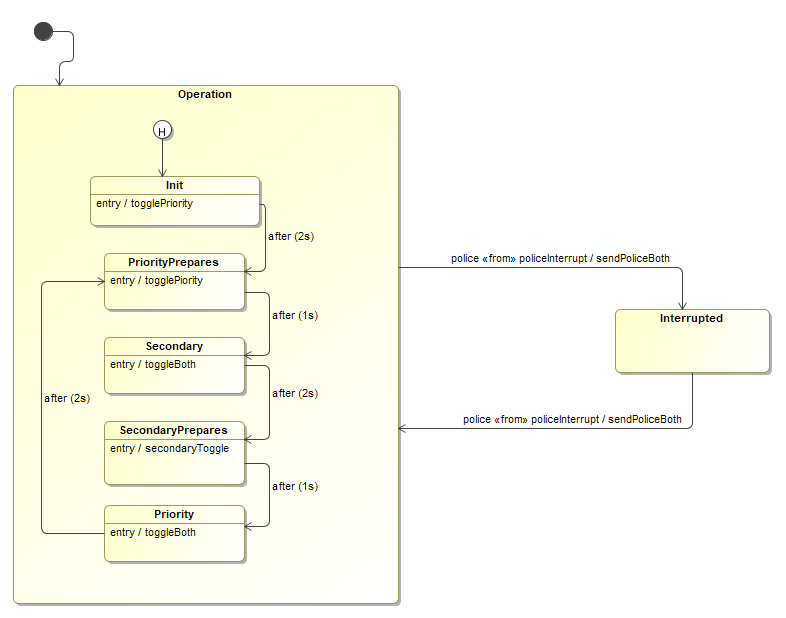
\includegraphics[width=90mm, keepaspectratio]{figures/preliminaries/statechart.png}
	\caption{Állapottérkép SysML-ben}
	\label{fig:statechart}
\end{figure}

Az állapotoknak van egy csoportja melyet pszeudo állapotoknak nevezünk. Ezek nem tényleges állapotai a rendszernek olyan értelemben, hogy a rendszer soha nem tartózkodhat ezekben mindig azonnal át kell lépniük belőle egy tényleges állapotba, viszont fontos szemantikai jelentéssel bírnak. A kezdő állapot mely fekete körként jelenik meg: 
\includegraphics[width=3mm, height=3mm]{figures/preliminaries/icons/initial.png}, egy régió belépési pontjai. Az állapotok mindig régiókban helyezkednek el, ezek tulajdonképpen állapotoknak egy olyan halmaza, amely halmazon belül mindig csak egy állapot lehet aktív, régiókból viszont lehet több is párhuzamosan. Így egy rendszernek lehet egyszerre több aktív állapota is régiónként viszont csak egy (a fork-joinra a dolgozat nem tér ki részletesen).

Pszeudo állapotok a \emph{History Statek} is. Ezek segítségével meg lehet jegyezni, hogy egy összetett állapot mely belső állapota volt aktív, így az állapotba visszalépve nem a belső régió kezdő állapota hanem az utolsó aktív állapot lesz újra aktív. \emph{History State}eknek két változata van \emph{Deep} és \emph{Shallow}. Előbbi egymásba ágyazott esetén minden régióba az utolsó aktív állapotba lép át, míg utóbbi csak a saját régiójának utolsó aktív állapotába. Jelölésük kör, benne "H"-val vagy "H*": 
\includegraphics[width=3mm, height=3mm]{figures/preliminaries/icons/history.png}. Létezik még választó pszeudo állapot (\emph{Choice state}) ez szintaktikailag egy rombuszként jelenik meg 
\includegraphics[width=3mm, height=3mm]{figures/preliminaries/icons/choice.png}. Ezzel lehet elágazásokat megvalósítani oly módon, hogy a kimenő állapot átmeneteken lévő őrfeltételek igazsága jelöli ki azt az élt ami tüzelhet (több igazra értékelt átmenet esetén nem determinisztikus módon az egyik tüzelhet). Választó állapotok esetén lehet egy őrfeltételben az \emph{else} kulcsszót használni, ilyenkor, ha nem volt más átmeneten igazra értékelődő őrfeltétel akkor ezen az átmeneten keresztül folytatódik a futtatás. A választó állapotból kimenő éleken nem lehet \emph{trigger}.

Az előbbieken kívül létezik még fork-join amivel párhuzamos futtatást lehet modellezni, csatlakozás (\emph{junction}), amivel élek vonhatók össze. Végső állapot (\emph{Final State}) ami a futtatás végét jeleni.


\subsection{A rendszer architektúrája}
Egy rendszer felépítését többféle szempont szerint is lehet modellezni. Ez egyik ilyen, hogy a rendszerünk milyen fizikai részekből áll és ezek között mi a kapcsolat, de fel lehet funkciók szerint is bontani. Utóbbit a rendszer funkcionális architektúrájának nevezzük.

Egy rendszer funkcionális architektúráján olyan modelleket értünk amelyek ennek a logikai felépítését írják le azaz, hogy milyen funkciói vannak a rendszernek, ezek hogyan kapcsolódnak egymáshoz. Jelen esetben ezeket a modelleket a rendszer állapotgépének a dekomponálására használjuk. Tehát van egy összetett rendszerünk melyeket funkcionális egységekre tudunk bontani úgy, hogy minden funkcionális egység állapot alapú viselkedések összessége. A komponensek képesek egymással kommunikálni és egymás viselkedését ezáltal befolyásolni.

A rendszert két szinten tudjuk modellezni: komponens definíciók és ezek kompozíciója, illetve ezeknek a kapcsolatai és belső szerkezete szerint. Előbbiek blokkok formájában jelennek meg és SysMLben Blokk definíciós (Block Definition) vagy BDD diagramokon jelennek meg A tartalmazásokat pedig \emph{Composition} élekkel tudjuk modellezni. Azt, hogy a blokkon belüli részek (\emph{Part}) hogyan kapcsolódnak egymáshoz Internal Block Diagramok (IBD) tartalmazzák. A részek közötti kapcsolatot konnektorok írják le. Ezek jellemzően portokon keresztül kötik össze a részeket. A portok tekinthetők egy adott blokk interfészének is.

A dolgozat elkészítésénél kétféle blokkot különböztetek meg. Azokat melyek állapotgépeket definiálnak és nem bonthatók részekre ezeket állapot blokkoknak nevezem. Illetve olyan blokkokat melyen részekre bonthatók, de nem definiálhatnak saját állapotgépet, ezeket pedig kompozit blokkoknak.

\section{MagicDraw}

A MagicDraw egy modellező eszköz melyet a NoMagic fejlesztett elsősorban UML modellek készítésére, bár talán inkább a SysML modellezés vált meghatározóvá. Ahhoz, hogy SyML-ben is tudjunk modelleket készíteni egy beépülő modulra van szükségünk (kivéve ha Cameo System Modellert használunk ami a SysML pluginnal integrálva szállít). A MagicDraw az iparban egy egyre inkább elterjedt eszköz. Szigorúan követi az UML és SysML szabványt.
Az modellezőeszköz gazdag funkcionalitással rendelkezik mint fejlett felhasználói interfész (\refstruc{fig:md-gui}), validációs motor - ami képes akár futásidőben a felhasználók által készített szabályok futtatására is, sablon alapú kódgenerátor és még sok egyéb. Ezen felül a funkcionalitás beépülő modulok segítségével bővíthető.

\begin{figure}[!ht]
	\centering
	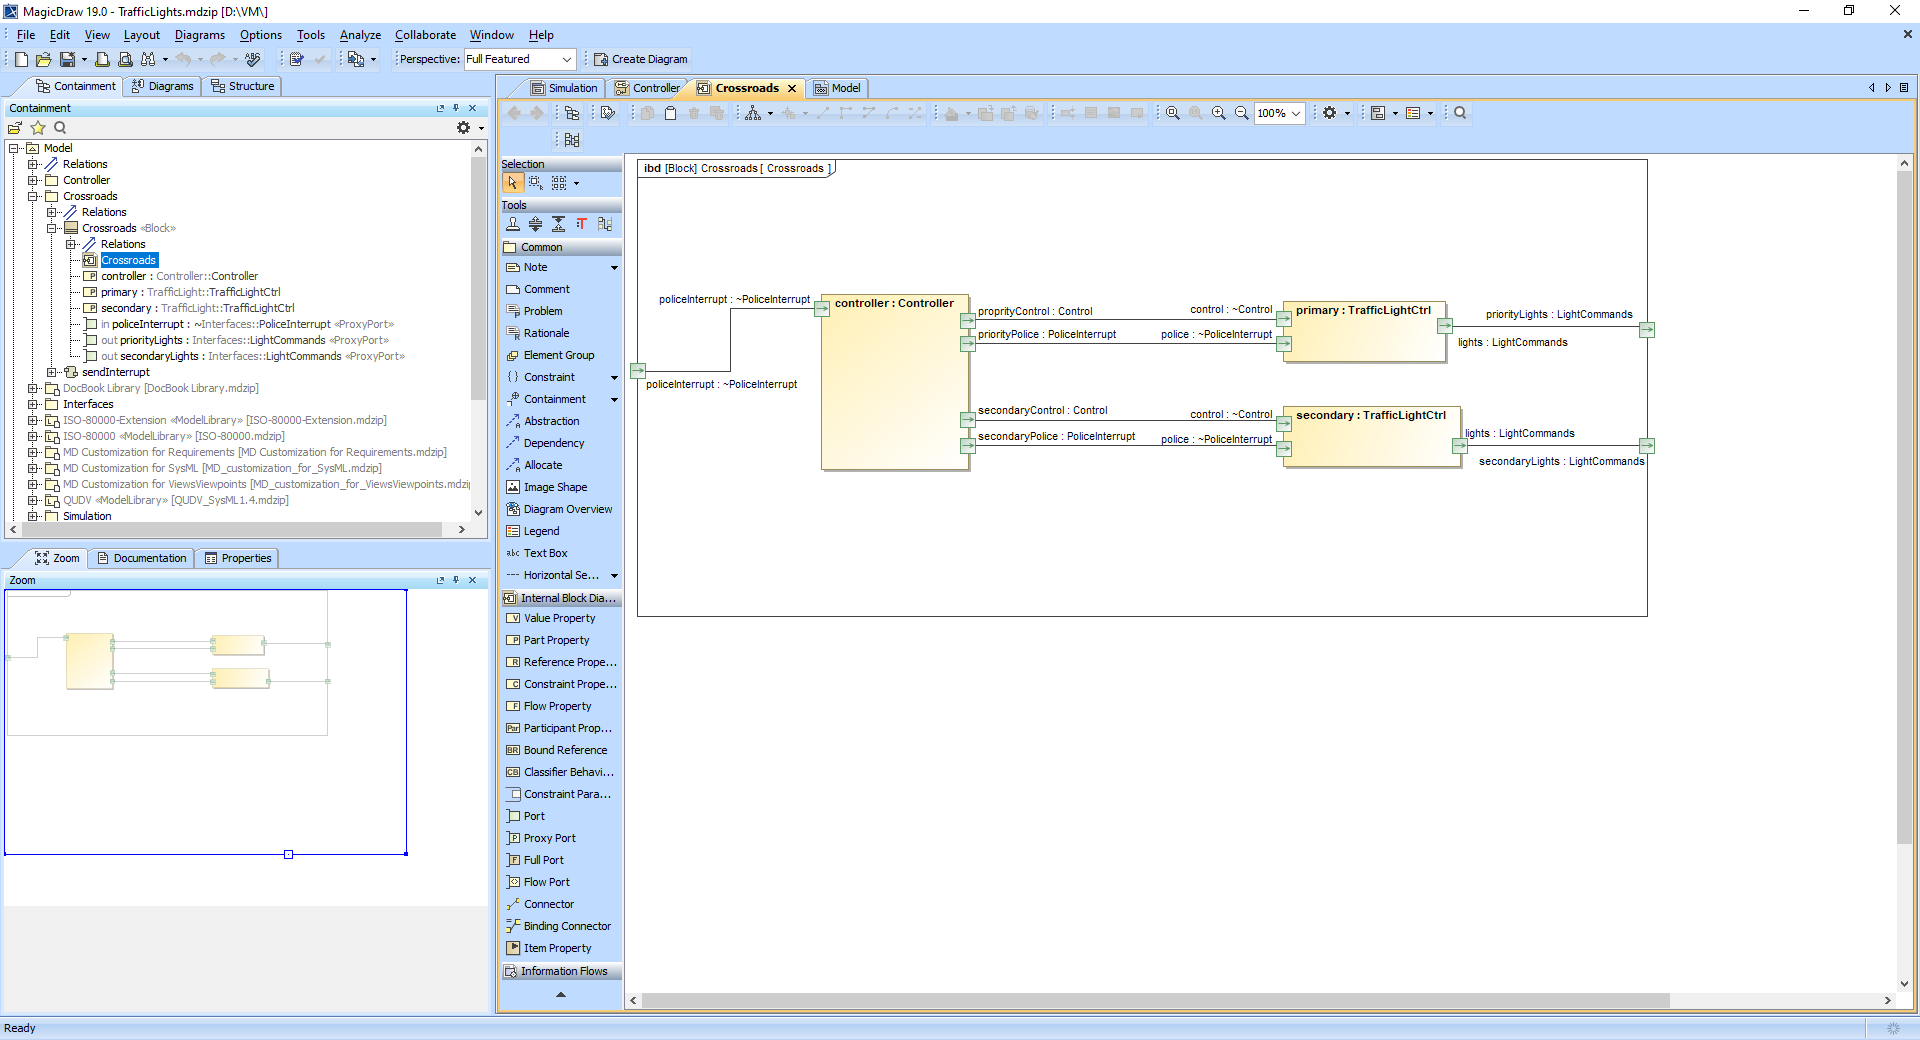
\includegraphics[width=140mm, keepaspectratio]{figures/preliminaries/md-gui.png}
	\caption{MagicDraw felhasználói felülete}
	\label{fig:md-gui}
\end{figure}

MagicDrawhoz lehetőségünk van saját plugin fejlesztésére is, amik lehetővé teszik számunkra, új funkcionalitás integrálását az eszközben illetve modellek manipulálását is. A feladatot is egy ilyen plugin fejlesztésével oldottam meg.


\section{Modelltranszformációk}

Az ipari standardok mellett sok speciális modellezési nyelv is létezik, amelyek megannyi céllal és az ezeket használó eszközökkel jöttek létre. Ezek között vannak magas absztrakciójú általánosabb nyelvek és alacsony szintűek is amik egy része olyan formalizmusokra épül amik felett bizonyos problémákra matematikai eszközökkel tudunk megoldást keresni.

A modellvezéreltség egyik alapötlete, hogy különböző modellekből származtatni tudunk más modelleket feltéve, hogy elegendő információ áll rendelkezésünkre a konverzió elvégzéséhez. Ezt a fajta származtatást például modell transzformációk segítségével tudjuk végrehajtani. A modelltranszformációk használata lehetővé teszi, hogy ne csak azokat a technológiákat használjuk modellünk feldolgozására melyek speciálisan az adott modellezési nyelvhez készültek hanem a modelleket megpróbáljuk átalakítani - lehetőleg a szemantikai tartalom megőrzésével és automatizáltan - egy olyan modellezési nyelvre amelyhez már létezik az általunk használni kívánt funkcionalitást támogató technológia.

Ezen felül dokumentumokat is tudunk származtatni a modellekből a kódgenerálás tulajdonképpen ennek egy speciális esete. Az sem ritka, hogy a származtatások több lépésen és modellen keresztül történnek. A kód generálásnál maradva a generált kód is egy modell amit általában egy fordítónak valamilyen futtatható állománnyá kell alakítani.


\section{Felhasznált technológiák}

Ebben az alfejezetben röviden kitérek azokra a tényleges  technológiákra, amelyekre a feladat elvégzése során használtam, mint például a VIATRA, a kiindulási alapot szolgáltató MagicDraw plugin és a Gamma.

\subsection[]{VIATRA\footnotemark}
\footnotetext{https://www.eclipse.org/viatra/}

A VIATRA egy keretrendszer mely lehetővé teszi eseményvezért modell transzformációk fejlesztését \cite{bergmann2015viatra}. Ehhez egy inkrementális modell lekérdezéseket leíró nyelvre a VIATRA Query Language-re (\refstruc{fig:vql}) támaszkodik. A létrehozott transzformációkat egy reaktív Query Engine futtatja és tartja karban.

\begin{figure}[!ht]
	\begin{lstlisting}
	pattern StateMachines(stateMachine: StateMachine, name: java String){
	    StateMachine.name(stateMachine, name);
	}
	
	pattern ParametersInStateMachine(stateMachine: StateMachine, parameter: Parameter){
    	StateMachine.ownedParameter(stateMachine, parameter);
	}
	
	pattern RegionsInRegion(container: Region, region: Region){
	    Region.subvertex(container, vertex);
    	State.region(vertex, region);
	}
	\end{lstlisting}
	\caption{Példa: VIATRA Query Language}
	\label{fig:vql}
\end{figure}


A VIATRA használata jelentősen megkönnyíti a modellekkel való munkát, bár én elsősorban a modell lekérdezés részére támaszkodtam a dolgozat elkészítése alatt. MagicDraw-ban egy pluginon keresztül van lehetőség VIATRA használatára melyet V4MD-nek hívnak. A plugin egy Query Engine-t biztosít számunkra per projekt. Ezen keresztül tudunk lekérdezéseket és transzformációkat regisztrálni. A V4MD leveszi a vállunkról a terhet az engine életciklus menedzsmentjét illetően. A VIATRA hátránya lehet azonban, hogy nagyon nagy modelleket komplex lekérdezések esetén a memóriaigénye elég jelentősre duzzadhat a háttérben, cserébe viszont az inkrementális működésnek köszönhetően a lekérdezések már csak a VIATRA által karbantartott táblázatokból való kiolvasás ezért költségül elhanyagolható. Éppen ezért olyan esetekben érdemes használni, amelyek kellően gyakran futnak és gyorsan van szükség az eredmény meghatározására mint például a futás idejű validáció.

\section{MagicDraw állapottérkép verifikációs plugin}

Ebben az alfejezetben bemutatom azt a SysML állapottrékép verifikációs eszközt, mely korábbi egyetemi munkám eredményeként képes volt MagicDraw modellek ellenőrzésére. A funkció megvalósításához a \emph{Gamma Statechart Composition framework} nevű keretrendszert használtam fel.

\subsection{Gamma Statechart Composition Framework \cite{DBLP:conf/icse/MolnarGVMV18}}

A Gamma Statechart Composition Framework (továbbiakban Gamma) egy állapottérkép modellező keretrendszer Eclipse felett ami integrálja a YAKINDU-t, de ezen felül saját nyelveket definiál nem csak állapottérkép leíráshoz, hanem ezek kompozíciójának modellezéséhez, akciók és őrfeltételek leírásához. Gammával a felhasználónak lehetősége van modellek formális verifikációját elvégezni, az eredményből pedig teszt kódot generálni, futtatható kód mellett.

A verifikáció eredményeként előálló időzítéseket és lépéseket visszavezeti a modellbe. Ezt Back-annotationnek nevezzük. Ezekhez szintén definiált egy nyelv, mely lehetővé teszi ezek dokumentálását.

A dolgozat elkészítése során nagy mértékben támaszkodtam a Gamma nyújtotta lehetőségekre. Ezt a Gamma mint egy köztes nyelv használatával érem el úgy, hogy modell transzformációk segítségével megvalósítok SysML-Gamma leképzést. A Gamma a formális verifikáció elvégzéséhez az UPPAAL nevű eszközt használja. Ez időzített automatákon tudja elvégezni a formális verifikációt (\refstruc{fig:gamma}). Ezeket a Gamma szintén modell transzformációk segítségével állítja elő, összekapcsolva a mérnöki modelleket matematikai modellekkel.
\begin{figure}[!ht]
	\centering
	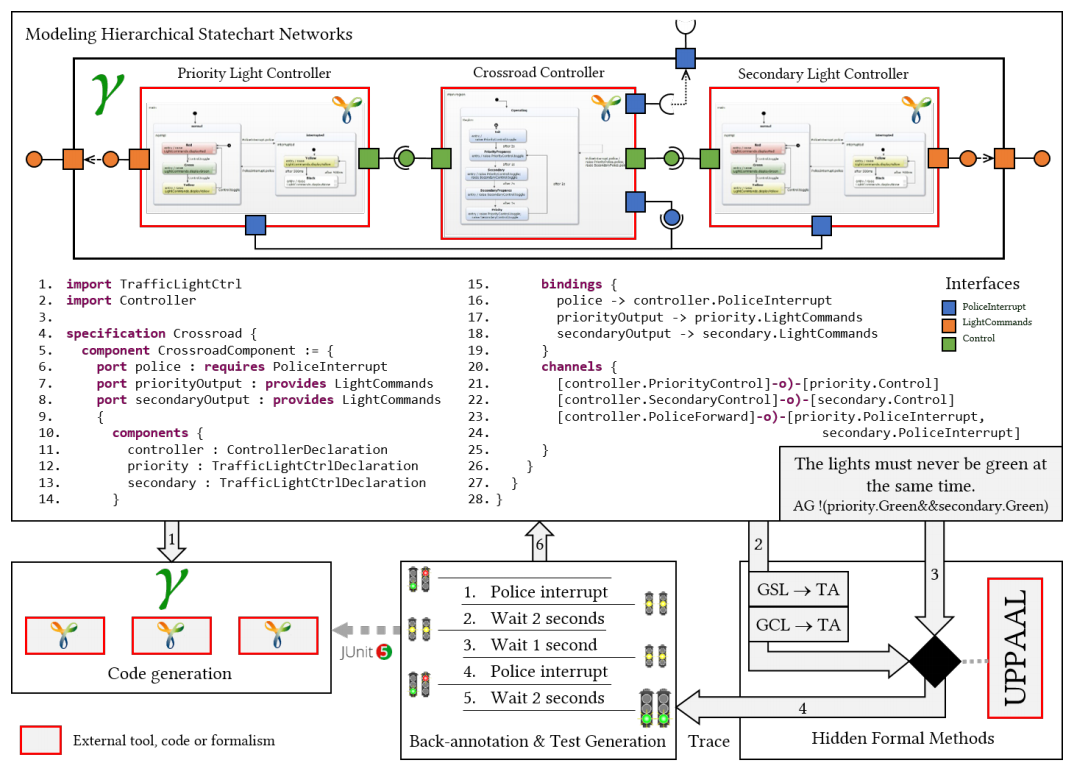
\includegraphics[width=140mm, keepaspectratio]{figures/preliminaries/gamma.png}
	\caption[]{A Gamma Statechart Composition Framework\footnotemark}
	\label{fig:gamma}
\end{figure}
\footnotetext{Forrás: https://inf.mit.bme.hu/sites/default/files/publications/icse18.pdf}
\newpage
A Gamma nagy erőssége, hogy állapotgép kompozíciókat is lehet modellezni benne. A komponenseket végrehajtás szempontjából háromféle szemantika van megkülönböztetve.

\paragraph{Szinkron komponensek} melyek egy lépésen belül fogadnak eseményeket ezekre lépnek és elküldik az eseményeket, ezek viszont a következő iterációban fognak fogadásra kerülni a hozzájuk kapcsolódó komponensekben.

\paragraph{Kaszkád komponensek (Cascade Component)} ezek hasonlóan működnek, mint a szinkron komponensek, viszont ebben az esetben a kiküldött üzenetek ugyan abban az iterációban kerülnek fogadásra. Ebből kifolyólag az üzenet áramlásnak aciklikusnak kell lennie, hiszen egy lépés feldolgozása végtelen ciklusba kerülne.

\paragraph{Aszinkron komponensek} Az események feldolgozása aszinkron módon, üzenet sorok kiolvasásával történik. Állapottérkép definíciók alapból szinkron szemantikával bírnak, így ahhoz hogy asszinkron szemantikával ruházzuk fel őket be kell csomagolni őket egy \emph{Wrapperbe}. Ez definiálja számukra az üzenet sort is.


\subsection{MagicDraw - Gamma transzformáció}

A MagicDraw beépülő modul fő célja SysML állapottérképek formális verifikációja. A Gamma képes állapotgépek ellenőrzésére ezek viszont a Gamma saját nyelvén kellenek, hogy legyenek definiálva. Modell transzformációk segítségével azonban lehetőségünk nyílik Gamma modellek származtatására SysML modellekből és ezáltal ellenőrizni őket.

Ez a származtatás vagy modell transzformáció képezi az ötlet alapját (\refstruc{fig:preliminaries-md-g}). A kihívás pedig az két nyelv közötti szemantikai különbségek feloldása illetve az elemek megfelelő egymáshoz rendelésének megtervezése és végrehajtása.

\begin{figure}[!ht]
	\centering
	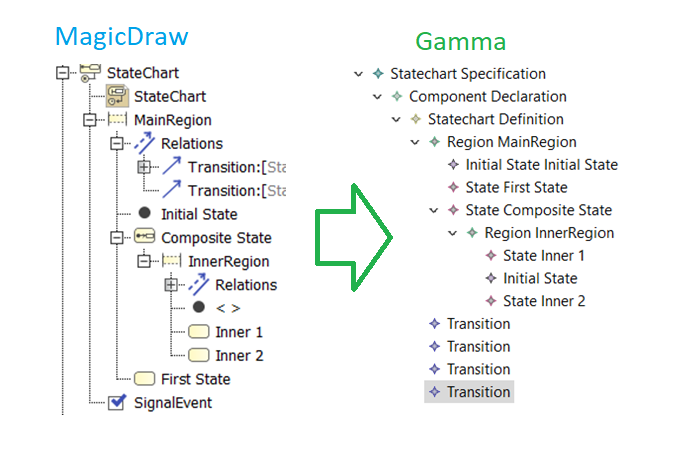
\includegraphics[width=150mm, keepaspectratio]{figures/preliminaries/md-g.png}
	\caption{Példa: egy modell transzformációra MagicDrawról Gammára}
	\label{fig:preliminaries-md-g}
\end{figure}

\subsection{Verifikáció menete}

A verifikáció elvégzése a MagicDraw beépülő modulban négy lépésből áll: 
\begin{itemize}
	\item MagicDraw modellek Gammává transzformálása
	\item Gamma modellek \uppaal\ modellé transzformálása (ezt a Gamma keretrendszer végzi el)
	\item tulajdonságok ellenőrzése UPPAAL segítségével
	\item Eredmény megjelenítése
\end{itemize}
Ezt a folyamatot \refstruc{fig:preliminaries-verif} szemlélteti. A Gamma által elvégzett lépéseket a zöld "Gammák" jelölik a modellben. Az ábrán a verifikációt a "Módosított Query Generátor" kezdeményezi, mely szintén a "Gamma" jelölést kapta. Ennek oka, hogy a beépülő modul ezen verziójában az ellenőrizendő tulajdonságok megadása még nem volt kiforrott ezért egy a Gamma keretrendszerből átemelt megoldás segítségével lehetett ezeket megadni és a verifikációt kezdeményezni. 

\begin{figure}[!ht]
	\centering
	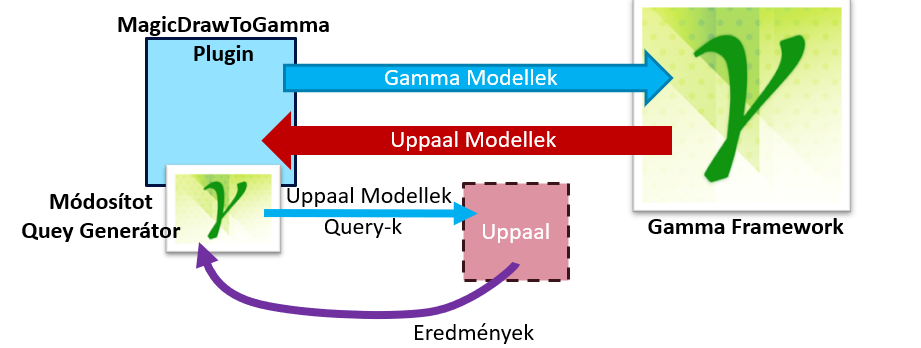
\includegraphics[width=150mm, keepaspectratio]{figures/preliminaries/concept.png}
	\caption{Verifikáció menete a pluginban}
	\label{fig:preliminaries-verif}
\end{figure}

\subsection{Őrfeltételek, akciók}

SysML nem definiál saját nyelvet őrfeltételek és akciók végrehajtásához. Míg akciókat tudunk modellezni bármilyen viselkedést leíró modell segítségével, addig az őrfeltételeket jellemzően valamilyen szöveges nyelvtannal szokás megadni.

Ahhoz, hogy a modell ellenőrzést végre lehessen hajtani ezeknek a Gamma számára érthető kifejezéseknek kell lenniük. A pluginnak ez a verziójában ezért minden őrfeltételt és akciót a Gamma által biztosított nyelvtan segítségével kellett megírni. Ez abból a szempontból nem szerencsés, hogy ez nem egy olyan elterjedt nyelv, mint például a javascript amit a MagicDraw támogat, továbbá nem áll még rendelkezésre olyan interpreter a MagicDraw-ban ami lehetővé tenné ezek futtatását ami elengedhetetlen többek között a modellek szimulációjához.


\section{Xtext}

Az Xtext egy keretrendszer amivel programozási nyelveket és egyéb szakterület specifikus nyelveket lehet készíteni, melyek szöveges formában manifesztálódnak. Ezeket valamilyen már meglévő modellezési nyelv egy konkrét szintaxisaként érdemes készíteni. Ez azt jelenti, hogy egy szövegesen megadott leírás elemeket és ezek kapcsolatait írja egy metamodellnek megfelelően.

Az Xtext nyelvtanok készítéséhez egy erős nyelvtan leíró nyelvet kínál. Az ezzel leírt nyelvtanhoz pedig teljes infrastruktúrát generál mint: \emph{parser}, \emph{linker}, típus ellenőrző, fordító. Ezen felül Eclipses környezetben a szerkesztéshez kapunk szintaxis kiemelést, \emph{content assist}ot.

MagicDraw-ban is ki tudjuk használni az Xtextben rejlő lehetőségeket és akár saját kiértékelő motort is tudunk írni, az általunk létrehozott nyelvtanokhoz. Sajnos a MagicDraw beépített szerkesztőjében elesünk olyan hasznos felhasználói funkcióktól mint a \emph{content assist} vagy a szintaxis kiemelés. Erre megoldást jelenthet az Xtext language szerver támogatásának a kihasználása a dolgozat azonban ennek a vizsgálatára nem tér ki.

Az Xtext használatára a dolgozat elkészítése során két helyen volt szükségem. Az egyik az őrfeltételek \emph{parse}olása, a másik pedig külön kérésre egy olyan export funkció integrálása ami XMI helyett a Gamma saját nyelvtanára sorosítva képes modelleket kimenteni.




\chapter{Plugin továbbfejlesztése}

Ebben a fejezetben ismertetem a beépülő modulon végzett továbbfejlesztéseket melyeket a mesterképzés során végeztem. 

\section{Fejlesztés céljai}

A fejlesztés során hozott alkalmazott megoldások áttekintése előtt érdemes végigvenni, hogy mik is voltak a fejlesztés fő céljai és mi volt ezeknek a motivációja.

\subsection{Funkcionális dekompozíció transzformálása}
Egy rendszert állapotait és állapotváltásait le lehetne modellezni egy mindent tartalmazó állapotgéppel, párhuzamos régiókkal és egyéb modellezési megoldásokkal. Ahogy a modell mérete nő a funkcionalitást érdemes feldarabolni és részenként modellezni. Ez nem csak az áttekinthetőséget segíti, de megkönnyíti a modellen való csapatmunkát is a mérnökök számára hiszen a szétbontott részeket külön, egymástól független lehet modellezni, majd ezeket összekapcsolni.

Szerencsére a Gamma erre a problémára is megoldást kínál, támogatja az állapot dekompozíció modellezését és formális verifikációját.

\subsection{Eredmények megjelenítése}
Fontos kérdés, hogy a formális verifikáció eredményét milyen formában kívánjuk megjeleníteni a mérnökök számára. A plugin eddigi verziója csak arra a kérdésre tudott választ adni, hogy teljesülnek-e a modellel szemben támasztott megkötések vagy sem.

Az \uppaal és a Gamma is képes sokkal részletesebb választ adni. Ezt a Gamma Back-annotation formájában teszi azaz a verifikációban előállt időzítések és lépéseket visszavezeti az eredeti modellbe. Ehhez a Gamma egy elég jól értelmezhető nyelvtant definiál, azonban a SysML-t jellemzően rendszermérnökök használják akik inkább a diagramokat mint a szöveges leírásokat preferálják általában.

A Back-annotationt úgy is lehet interpretálni mint lépések egy sorozatát, amelyek szinkron esetben egymást jól meghatározható sorrendben követik. Ezt leginkább szekvencia diagramokon lehet ábrázolni. Ezen felül ami miatt még a szekvencia diagram tűnik a legkézenfekvőbb megjelenítési megoldásnak az a MagicDraw, illetve a Cameo Simulation toolkit. Ez ugyanis képes szimulációt rögzíteni szekvencia diagramok formájában (\refstruc{fig:md-cameo-rec})) és ezeket újra lejátszani. A cél tehát olyan szekvencia diagramok előállítása úgy minthogyha a szimulátort használva találtuk volna meg a hibautakat, így ezekről nem csak egy jól áttekinthető megoldást kapunk szekvenciák formájában, hanem ezek szimulálhatók is lesznek Cameo Simulation Toolkit segítségével.

\begin{figure}[!ht]
	\centering
	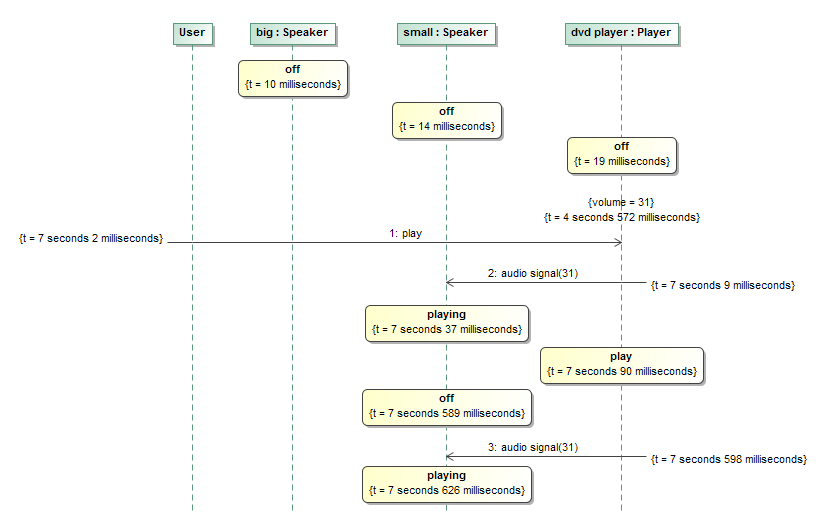
\includegraphics[width=140mm, keepaspectratio]{figures/contribution/md-cameo-rec.png}
	\caption[]{Rögzített szimuláció szekvencia diagramon\footnotemark}
	\label{fig:md-cameo-rec}
\end{figure}

\footnotetext{Forrás: https://docs.nomagic.com/display/CSTD184/Recording+simulation+as+a+Sequence+diagram}

\subsection{Követelmények definiálása}

A formális verifikáció elvégzéséhez a modelleken felül meg kell tudnia a felhasználónak azokat a kérdéseket melyekre választ szeretne kapni a modell ellenőrzése során. Ezek jelen esetben a "Kerülhet-e a rendszer adott állapotba" illetve "Adott állapotból el tud-e jutni egy másikba" típusúak jellemzően. Az \uppaal-ban ezeket temporális logikai kifejezések segítségével tudjuk megtenni \uppaal Queryk formájában ezért ezeket az ellenőrzés során elő kell állítanunk.

Eredetileg szándékoztam erre egy saját nyelvtant is fejleszteni, de a Gammához időközben készült egy úgynevezett \emph{Property Language} és ez ennek az \uppaal-ra transzformáló funkciója és végül ezt használtam fel.

\subsection{Validáció}

A fejlesztés során hozott számos döntés megköveteli, hogy a modellekre vonatkozzanak bizonyos jól-formáltsági kényszerek. Ezek egy része a Gammából örökölt. Például a \emph{Property Language} egy komponensen belül egy állapotra a régión keresztül tudunk hivatkozni (\emph{[component]+.region.state}). Ebből következik, hogy a régióknak a MagicDraw modellben nevet kell adni, illetve, hogy ezek egyediek legyenek egy állapottérképen belül.

A dolgozat célja egy validációs szabálykészlet létrehozása ami segít a felhasználóknak az eszköz helyes használatában.

\newpage

\section{Gamma UML profil}

A dolgozat elkészítéséhez pusztán a SysML nyelv nem volt elegendő ugyanis szükséges volt  a modellben is eltárolni  bizonyos információkat, mint például az ellenőrizendő követelmények, a Back-annotation, vagy éppen, hogy milyen kompozit szemantikát kívánunk érvényesíteni az adott modellekre.

Ezek információk modellezhetőségéhez készítettem egy MagicDraw profilt. Ez alapvetően három részből áll:

\begin{itemize}
	\item Kompozit szemantika
	\item Check modell
	\item Back-annotation modell
\end{itemize}

Az UML profil érdekessége, hogy tartalmazásokat csak megkötés szintjén \emph{Customization}on keresztül tudunk megadni. UML profil diagramon csak öröklést és \emph{tag}eket van lehetőségünk definiálni.



\subsection{Kompozit szemantika}

A Gamma háromféle komponens végrehajtási szemantikát biztosít a felhasználók számára. Ugyan ezt implicit módon is meg lehet határozni, például a kommunikáció típusából, mégis fontos lehet ezek egyértelmű jelölése. Ezért az UML profil (\refstruc{fig:comp-prof}) a SysML nyelvet kiegészíti néhány sztereotípiával melyek segítségével explicit jelölhetők, hogy milyen szemantikát szeretne a felhasználó érteni Blokkjain.

\begin{figure}[!ht]
	\centering
	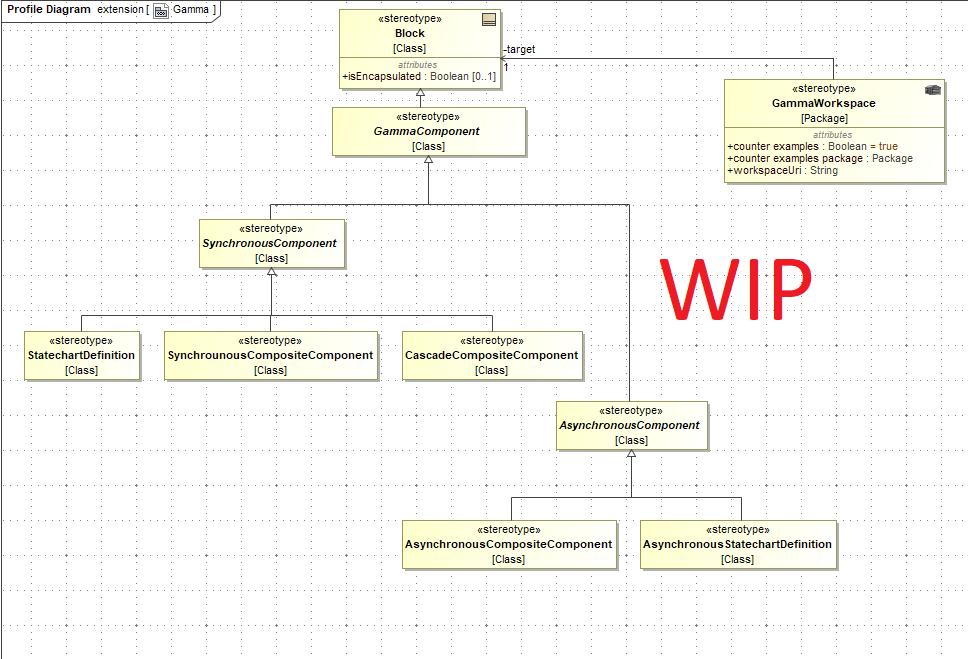
\includegraphics[width=150mm, keepaspectratio]{figures/contribution/profile.png}
	\caption{Szinkron, asszinkron szemantikát támogató UML profil}
	\label{fig:comp-prof}
\end{figure}

A sztereotípiák leszármaznak a Block sztereotípiájából, így lényegében lecserélik azt. Ennek előnye hogy szintaktikailag is asszinkron és szinkron blokkok fognak megjelenni a modelljeinkben. Viszont van egy nagyon nagy hátulütője is mégpedig az, hogyha már meglévő modelleken szeretnénk használni az eszközt ezekhez hozzá kell nyúlni, amihez például elosztott környezetben nem biztos, hogy egyszerű. Ami mégis elfogadhatóvá teszi ezt a plugin jelenlegi iterációjának kapcsán az az őrfeltételek és az akciókra vagy akár az interfészekre vonatkozó megkötések amik - sajnálatos módon - jó eséllyel megkövetelik a modell módosítását.

Egy alternatív megoldás az lehetne, hogy a sztereotípiákat valamilyen él például \emph{Dependency} segítségével rendeljük az egyes komponens definíciókhoz, vagy akár partokhoz. Ez megoldást nyújthat arra a problémára is, hogyha a modell egyes részei külső könyvtárból jönnek, vagy nincs hozzáférésünk hozzájuk.


\subsection{Check modell}

Ahhoz, hogy a formális verifikáció végrehajtható legyen ki kell választani, hogy milyen modelleket szeretnénk ellenőrizni és ezeken milyen követelményeket. Az formális verifikációt modell elemeken keresztül lehet paraméterezni.

Az elképzelés szerint a felhasználó \emph{Workspace}eket hoz létre. Ezek hivatkoznak a felhasználó számítógépén egy könyvtárra melyet az infrastruktúra sajátosságából adódó háttértárra kimentendő modelleket tárolására használok. Ezen felül rajta keresztül kell behivatkozni az ellenőrizendő modellt a projektből.

A modell transzformációk során \emph{Trace}k keletkeznek. Ezek alapján lehet visszakeresni, hogy mely a MagicDraw - Gamma transzformáció során milyen leképzések történtek. Ezek valójában UML propertyk egy \emph{Class}on belül melyeknek a neve egy azonosító amivel a Gamma modell egy kisorosított XMI fájlban lévő elemei vannak hivatkozva. A \emph{property}kből egy \emph{Trace} él mutat a megfelelő MagicDraw elemekre. A kisorosított XMI ugyan ezen \emph{Class} modell elemekhez mint \emph{Comment} vannak hozzárendelve, innen lehet őket kiolvasni.

A követelményeket \emph{GammaProperty} segítségével lehet megadni a Gamma által definiált Property nyelvtan segítségével. Az ezek ellenőrzéséből származó Back-annotaion modellek is a \emph{Workspace}ben helyezkednek el. A modell elemei a következők:
%TODO Update
\begin{itemize}
	\item \textbf{GammaWorkspace} \newline
	Transzformációk és ellenőrzések kezelésére szolgáló MagicDraw projektben tárolt modell.
	\newline
	\textit{Attribútumok:}
	\subitem Target: InstanceSpecification[1]: transzformálandó modell
	\subitem WorkspaceUri: String: egy elérési út a felhasználó egy könyvárához
	\subitem Counter examples: Boolean: Back-annotation engedélyezése
	
	\item \textbf{GammaCheck} \newline
	\emph{GammaProperty}k konténere
	
	\item \textbf{GammaProperty} \newline
	Egy a modellel szemben támasztott követelmény a saját nyelven
	\newline
	\textit{Attribútumok:}
	\subitem body: String[1]: saját nyelven írt kifejezés

	\item \textbf{GammaWorkspaceFile} \newline
	Hivatkozás egy Gamma modellre a háttértáron. A modell elem neve a fájl elérési útja.
	
	\item \textbf{MD2G\_Trace} \newline
	Egy megfeleltetés a MagicDraw és Gamma modellek között. A MagicDraw elemre egy Trace él mutat, a Gammabeli modell elem pedig EMF hivatkozás formájában kerül tárolásra.
	\newline
	\textit{Attribútumok:}
	\subitem URIFragment: String[1]: hivatkozás EMF-es modell elemekre
	
	
\end{itemize}

\subsection{Back-annotation modell}
A back-annotation modell feladata visszacsatolni az eredeti modellbe a valamilyen külső, jellemzően szimulátorból származó időzítési adatokat. A Gamma is készít egy ilyen modellt. A megoldás amit kidolgoztam Gamma modell egy MagicDraw specifikus változatának létrehozásából és egy Gamma-MagicDraw transzformáció megtervezéséből és megvalósításából állt. Az UML profil egy szakterület specifikus nyelvet definiál. Elemei pedig a következők:

\begin{itemize}
	\item \textbf{ExecutionTrace} \newline
	Egy kompozit komponens végrehajtása. \textit{Steppeket} azaz lépéseket tartalmaz, illetve a végrehajtás végén állhat egy lépésekből álló ciklus.
	\newline
	\textit{Attribútumok:}
	\subitem component: InstanceSpecification[1]: kompozit komponens példánya a modellben
	\subitem steps: Step[1..*]: lépések
	\subitem cycle: Cycle[0..1]: lépésekből álló ciklus amire a végrehajtás futhat
	
	\item \textbf{Step} \newline
	A végrehajtás egy lépése. Két részből áll egy \textit{Act} részből, ami a végrehajtódott műveleteket írja le és egy \textit{Assert} részből, ami a lépésben elért állapotot írja le.
	\newline
	\textit{Attribútumok:}
	\subitem actGroup: ActGroup[0..1]: műveletek konténere
	\subitem assert: Assert[1]: lépés során beálló állapotok
	
	\item \textbf{ActGroup} \newline
	\textit{Actok} konténere a \textit{Steppen} belül. Csak áttekinthetőségre szolgál.
	\newline
	\textit{Attribútumok:}
	\subitem acts: Act[0..*]: műveletek konténere
	
	\item \textbf{Act} \newline
	Absztrakt sztereotípia. Egy végrehajtott művelet.
	
	\item \textbf{ComponentSchedule} \newline
	Komponensen egy kör végrehajtása (üzenetek kiolvasása az üzenetsorokból, állapotok léptetése)
	
	\item \textbf{TimeElapse} \newline
	Végrehajtás várakoztatása bizonyos ideig.
	\newline
	\textit{Attribútumok:}
	\subitem value: Integer: várakozás ideje milliszekundumban
	
	\item \textbf{RaiseEventAct} \newline
	Egy esemény elküldése a komponens példánynak.
	\newline
	\textit{Attribútumok:}
	%TODO ez itt biztosan válozik majd
	\subitem referencedAction: Behavior: eseményt küldő viselkedés.
	
	\item \textbf{InstanceState} \newline
	Absztrakt. Az egyes példányok, partok állapotainak leírása.
	\newline
	\textit{Attribútumok:}
	\subitem referencedPart: PartProperty: hivatkozott komponens példány
	
	\item \textbf{InstanceVariableState} \newline
	Egy változónak egy állapota.
	\newline
	\textit{Attribútumok:}
	\subitem referencedVariable: Property: hivatkozott változó
	\subitem value: ValueSpecification: hivatkozott változó értéke
	
	\item \textbf{InstanceStateConstant} \newline
	Az állapot gép egy állapota.
	\newline
	\textit{Attribútumok:}
	\subitem referencedState: State: hivatkozott állapot konstans
\end{itemize}

A \refstruc{fig:contribution-trace-profile} az UML profilt, a \refstruc{fig:contribution-trace-customization} pedig ennek a customizationjét mutatja.

\begin{figure}[!ht]
	\centering
	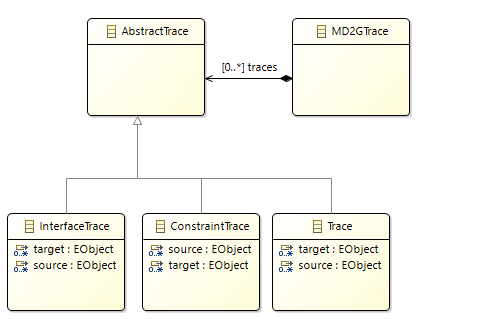
\includegraphics[width=90mm, keepaspectratio]{figures/contribution/trace-model.png}
	\caption{Back-annotation UML profilja}
	\label{fig:contribution-trace-profile}
\end{figure}

\begin{figure}[!ht]
	\centering
	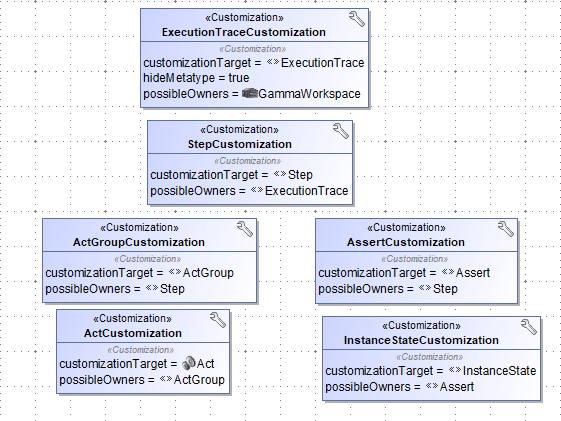
\includegraphics[width=90mm, keepaspectratio]{figures/contribution/trace-profile.png}
	\caption{Back-annotation customization modellje}
	\label{fig:contribution-trace-customization}
\end{figure}
 
 \newpage


\section{Kompozíciók transzformációja}

Egy nagy komplex rendszert célszerű nem egyben, hanem részekre bontva modellezni majd a részek egymáshoz illesztéséből, komponálásából képezni a teljes rendszert. Állapottérképek dekomponálását azaz részekre bontását a Gamma is támogatja. A kihívás a SysML és a Gamma közötti megfeleltetések megválasztása oly módon, hogy a szemantika ne sérüljön. A megfeleltetés két szempontól kell vizsgálni, egyszer az elemek tartalmazási hierarchiái szerint, egyszer pedig a köztük modellezett kommunikáció szerint.



\subsection{Struktúra megfeleltetése}
A Gammában nyelvi szinten elkülönül az állapottérkép (StatechartDefinition) és a kompozit komponens (Composite Component) fogalma. Állapottérképek a modell hierarchia gráfjában a levelekben helyezkednek el. SysML esetében a minden Blokknak lehet viselkedése, jelen esetben állapottérképe. A megfeleltetés elvégzéséhez megkötést fogalmaztam meg mely kétféle blokkot enged meg. A viselkedéssel rendelkező blokkokat és azokat amelyek nem tartalmazhatnak viselkedést csak Part Propertyket. Tehát állapottérképek ebben a modellben is csak levelekben lehetnek.

\begin{figure}[!ht]
	\centering
	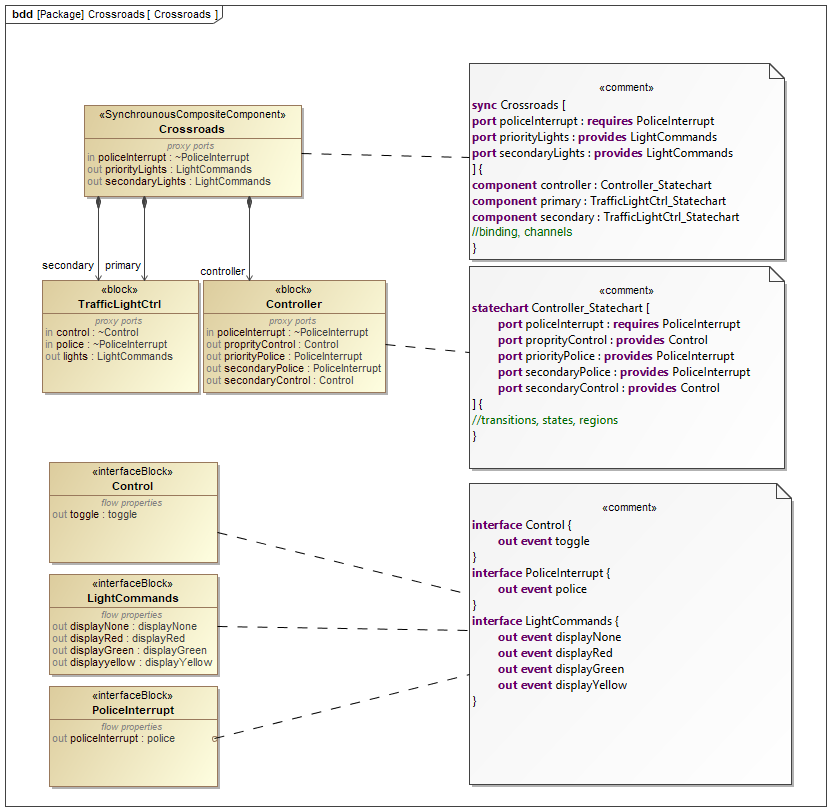
\includegraphics[width=140mm, keepaspectratio]{figures/contribution/md2g.png}
	\caption{Struktúra megfeleltetése}
	\label{fig:md2g}
\end{figure}

Az érdekes kérdés lehet, hogy ha egy magasabb szintű blokknak mégis lehetne viselkedése, azt szemantikailag hogyan kezelhetnénk. Elképzelhető olyan értelmezés, hogy ez a magas szintű állapottérkép a dekomponált részek együttes viselkedését írja le. Ez lehetőséget adna arra, hogy a magasabb és az alacsonyabb szintű viselkedés halmazt összehasonlítsuk működés szempontjából és ha nincsenek szinkronban akkor tervezési hibaként értelmezzük. Így a magasabb hierarchia szintek tulajdonképpen validálnák az alacsonyabb szinteket. Ennek a lehetőségnek a komolyabb kifejtése azonban nem célja a dolgozatnak.

\subsection{Kommunikáció megfeleltetése}

A Gammában a komponensek kommunikációja kimondottan az eseményvezérelt állapot alapú rendszerek sajátosságain alapul, azonban SysML-ben a kommunikáció leírása sokkal általánosabb és többféle módon is modellezhető. Éppen ezért a feladat elvégzése során az események és az interfészek modellezésére megkötéseket kellett megfogalmazni.
Az egyik ilyen megkötés szerint a portokban interfész blokkokat kell tipizálniuk és szinkron szemantika esetében operációkat definiálni, asszinkron esetben pedig szignálokkal tipizált \emph{Flow Property} formájában fel kell tüntetni milyen szignálok fogadására képes a blokk.

Az eseményeknek mindig specifikálniuk kell, hogy melyik porton várják az operáció hívását vagy szignál érkezését. Ez igaz az akciókra az ő esetükben azt kell specifikálni, hogy milyen porton keresztül történjen a küldés.

Portok közül csak a \emph{Proxy} portok támogatottak. Proxy portok iránya származtatott a \emph{Flow property} irányokból amik keresztül mehetnek rajta. Az irány az \emph{isConjugated} flag igazra állításával változtatható.

\section{CTL nyelvtan}

\section{Back-annotation transzformációja}

A Back-annotation egy általában szimulátor által biztosított időzítési adatok visszacsatolása az eredeti modellbe. Ahhoz, hogy MagicDrawban is el tudjuk tárolni ezeket az adatokat létre kellett hoznom egy UML profilt ami a Back-annotation modell metamodelljeként fog szolgálni.

A transzformáció iránya itt megfordul nem MagicDraw modellekből állítok elő Gamma modelleket hanem épp fordítva Gamma modelleket transzformálok MagicDraw modellekké.



\section{Szimuláció}

\section{Validáció}

\section{Példa} %TODO TBD

Ebben az alfejezetben bemutatom az eszköz használatát egy példamodellen. Ez a modell a Gamma tutorial csomagjában lévő közlekedési lámpákat tartalmazó modelljének SysML-be átemelt változata. A példán ismertetése közben bemutatom a az eszköz által támogatott modellezési módszertant is.

\subsection{A példamodel}

A modell három komponensből áll (\ref{fig:Crossroads} ábra): két a lámpákat irányító (\emph{primary}, \emph{secondary}) és egy az ezeket szinkronban tartó \emph{Controller} komponensből. A rendszernek van két kimeneti portja amellyel a két közlekedési lámpa jelzéseit tudja változtatni és rendelkezik egy bemeneti porttal amelyen keresztül a rendőrség \emph{Interrupted} ("Sárga villogó") állapotba tudja állítani a rendszert illetve vissza is tudja állítani a normál állapotba, ahol a piros - zöld - sárga jelzések váltakoznak a két lámpán mégpedig egymásnak ellentétesen.

\begin{figure}[!ht]
	\centering
	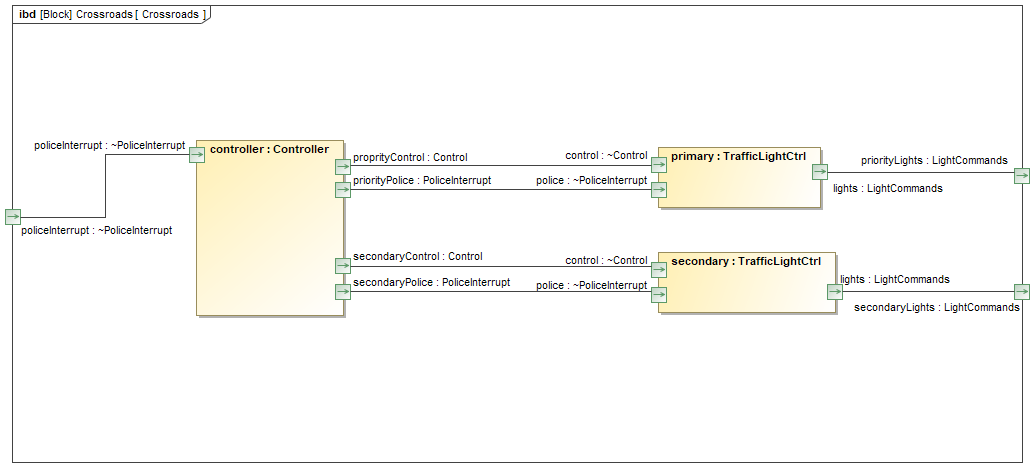
\includegraphics[width=15cm, keepaspectratio]{figures/contribution/Crossroads.png}
	\caption{Az útkereszteződés SysML modellje}
	\label{fig:Crossroads}
\end{figure}

A rendszer három interfészt definiál (\ref{fig:Interfaces} ábra): \emph{PoliceInterrupt}, \emph{Control}, \emph{LightCommands}. Ezek mindegyike \emph{Interface Block}ként kell, hogy megjelenjen a modellben, és minden az állapottérképeken használt \emph{Signal}hoz fel kell venni egy \emph{Flow Property}-t a megfelelő iránnyal. Jelen esetben ez a következőként jelenik meg. A \emph{Control} interfész tartalmaz egy \emph{Flow Property}-t \emph{out}, azaz kimenő iránnyal és egy 'toggle' nevű \emph{Signal}lal van tipizálva. Ez azért fontos mert az állapottérképen ezeket a \emph{Signal}okat kell majd használni. A \emph{LightCommands} négy kimenő \emph{Property}t tartalmaz. Ezek a \emph{displayNone}, \emph{displayRed}, \emph{displayGreed} és \emph{displayYellow} szignálokkal vannak tipizálva. A \emph{PoliceInterrupt} interfész csak egy \emph{Property}t tartalmaz \emph{out} iránnyal a \emph{police} szignálhoz.

\begin{figure}[!ht]
	\centering
	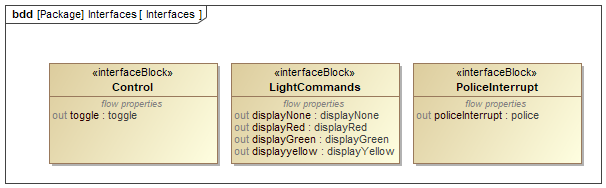
\includegraphics[width=15cm, keepaspectratio]{figures/contribution/Interfaces.png}
	\caption{Interfészek a modellben}
	\label{fig:Interfaces}
\end{figure}

Most, hogy már az interfészek és a portok le vannak modellezve el ezeket fel lehet használni az állapottérképek leírásához. A modell két állapottérképet definiál egyet a két lámpa controllerjéhez (\emph{LightCtr}-hez) és egyet a \emph{Controller}hez.

Tekintsük előbb a \emph{Controller} állapottérképére (\ref{fig:ControllerSM} ábra). Az állapotgép egy kompozit állapotból és ennek négy belső állapotából áll. \emph{Police Interrupt} hatására az állapotgép kilép a kompozit állapotból mindkét \emph{PoliceInterrupt} típusú portján küld egy-egy \emph{policeInterrupt} jelet, majd visszatér ugyan ebbe az állapotba. Amelyben a \emph{History State} miatt abból az állapotba kerül vissza amiben a kilépés előtt volt.

\begin{figure}[!ht]
	\centering
	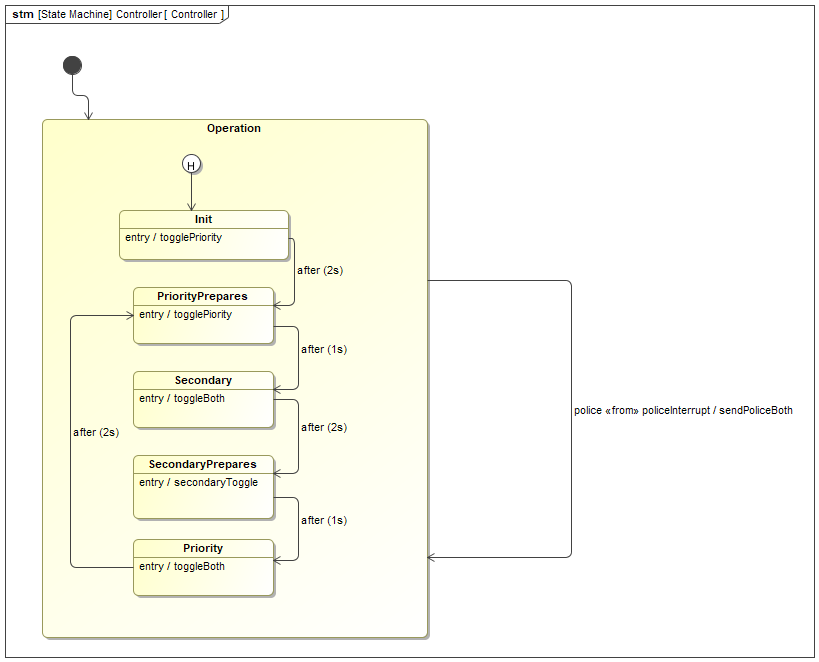
\includegraphics[width=12cm, keepaspectratio]{figures/contribution/ControllerSM.png}
	\caption{Controller állapotai}
	\label{fig:ControllerSM}
\end{figure}

Ami ennek az állapot átmenetnek a modellezése kapcsán izgalmas az \emph{Signal} küldésnek a módja. A plugin jelenlegi formájában ezt Activity diagrammal kell leírni \emph{Send Signal} akciók használatával. Ez jelen esetben egy két akciós \emph{Activity}t fog eredményezni, amelyben sorban a megfelelő portokon elküldésre kerülnek a szignálok (\ref{fig:activity} ábra).  A \emph{togglePriority}, \emph{secondaryToggle} és \emph{toggleBoth} \emph{entry action}ok hasonlóan vannak modellezve.

\begin{figure}[!ht]
	\centering
	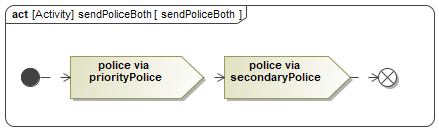
\includegraphics[width=12cm, keepaspectratio]{figures/contribution/sendPoliceBoth.png}
	\caption{\emph{Signal}ok küldése Activityel}
	\label{fig:activity}
\end{figure}

Amiről ennek az állapottérképnek a kapcsán még érdemes lehet beszélni ezek a bizonyos idő elteltével tüzelő átmenetek. Ezek a modellben \emph{Time Event}ként jelennek meg. Fontos hogy ezeknek a \emph{relative} attribútumát igazra kell állítani, hisz ez jelenti azt, hogy a forrás állapotba való belépéstől kell számítani az időt.

A teljesség kedvéért vizsgáljuk meg a másik állapottérképet is (\ref{fig:LightCtrlSM} ábra). Ez két kompozit állapotból áll. A \emph{Normál} a szokásos működést jelenti és a \emph{Red}, \emph{Green}, \emph{Yellow} állapotokból áll melyek a beérkező toggle szignálok hatására váltakoznak.
Az \emph{Interrupted} állapot a rendőrség által előidézett "sárga villogó" állapotot jelenti. Ebben a \emph{BlinkingYellow} és a \emph{Black} állapotok váltakoznak 500 milliszekundumonként.  

\begin{figure}[!ht]
	\centering
	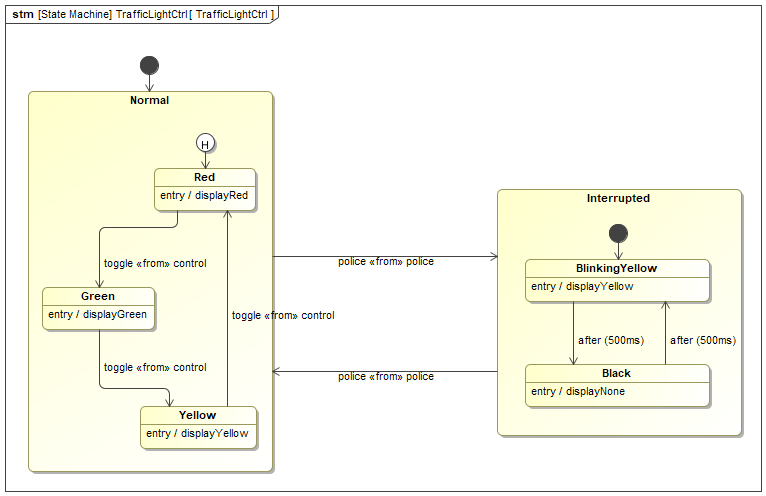
\includegraphics[width=12cm, keepaspectratio]{figures/contribution/TrafficLightCtrlSM.png}
	\caption{\emph{TrafficLightCtrl} állapottérképe}
	\label{fig:LightCtrlSM}
\end{figure}


\subsection{Transzformációk végrehajtása}

A modell összerakásánál egy dolog még nem lett lemodellezve, mégpedig, hogy melyik komponenst szemantikát szeretnénk alkalmazni. Jelen esetben a szinkron szemantikát szeretnénk. Ehhez jelen esetben elegendő a gyökér elem \emph{Block} sztereotípiáját a specifikusabb \emph{SynchronousCompositeComponent}re cserélni.
Most, hogy a komponens szemantika specifikálva van a modellek transzformálhatók és ellenőrizhetők.

Első lépésként létre kell hozni egy \emph{GammaWorkspace}t. Ez a modell elem fogja tárolni az ellenőrzés során szükséges adminisztrációs objektumokat. Azonban meg kell nevezni egy könyvtárat is a háttértáron amit ideiglenes fájlok tárolására fog a plugin használni. Ehhez egy \emph{Workspace Uri}t kell megadni ami egy abszolút elérési út egy tetszőleges könyvtárhoz. Az ellenőrizendő modellt a \emph{Target} mező megadásával lehet specifikálni.

\begin{figure}[!ht]
	\centering
	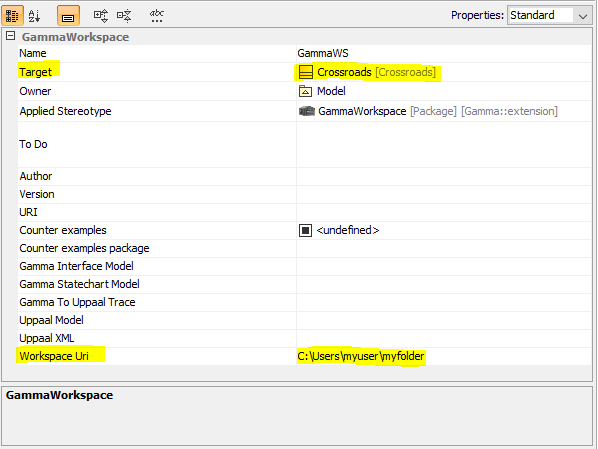
\includegraphics[width=7cm, keepaspectratio]{figures/contribution/GammaWS.png}
	\caption{\emph{GammaWorkspace} specifikációja}
	\label{fig:GammaWS}
\end{figure}


A kötelező mezők specifikálása után a \emph{Gamma Workspace}n nyitott gyorsmenüben a \emph{Gamma Transformation} menüpont alatt található akciók segítségével tudjuk a transzformációkat végrehajtani (\ref{fig:gamma-tra}). Az egymással függésben lévő lépések akkor válnak aktívvá, hogyha a bemenetük már előállt.

\begin{figure}[!ht]
	\centering
	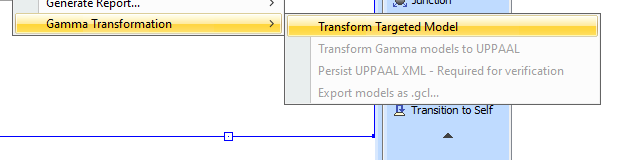
\includegraphics[width=10cm, keepaspectratio]{figures/contribution/GammaTransformation.png}
	\caption{Gyormenü elérése a transzformációkhoz}
	\label{fig:gamma-tra}
\end{figure}

Az akció végrehajtását követően két dolog történik. Először is megjelenik két \emph{GammaModel} sztereotípiával ellátott osztály elem, a transzformált interfészeknek és a komponenst modelleknek illetve állapotgépeknek. Másfelől a \emph{GammaWorkspace} \emph{Gamma Statechart Model} és a \emph{Gamma Interface Model} mezők ezekre fognak mutatni. A letranszformált modellek ezekhez a sztereotipizált osztályokhoz XMI formátumban kommentek formájában hozzá lesznek rendelve innen lehet őket \emph{EMF Resource}okba visszaolvasni amennyiben erre szükség van, így nem kell újra letranszformálni a modelleket.

Az osztályok belsejében továbbá létrejön jó pár \emph{property}. Ezek csomópont hivatkozások az XMI fájlok egyes elemeire. Belőlük pedig \emph{Trace} élek futnak melyek MagicDraw elemekre mutatnak. Ez az a visszakövethetőségi modell melynek segítségével tudjuk, hogy melyik Gamma elem milyen MagicDraw elemekből állt elő. Ezt \aref{fig:traces} ábra szemlélteti, ahol a \emph{Traced element} egy származtatott oszlop a \emph{Trace} élek cél elemei.

\begin{figure}[!ht]
	\centering
	\includegraphics[width=10cm, keepaspectratio]{figures/contribution/Traces.png}
	\caption{Elemek visszakövethetősége MagicDrawban (részlet)}
	\label{fig:traces}
\end{figure}

Következő lépés a az UPPAAL EMF speficikus modelljének előállítása  ez ehhez tartozó \emph{trace}kkel együtt amelyeket a Gamma majd a back-annotation előállításához használ majd. Ezeket a mostmár aktív "Transform models to UPPAAL" akció végrehajtásával tudjuk megtenni. Hasonlóan ez előbb szemléltetettekhez létrejön két sztereotipizált osztály egy az UPPAAL modellnek egy pedig az UPPAAL - Gamma \emph{traceknek}. A modellek ugyan úgy mint az előbb XMI formátumban az elemekhez lesznek kapcsolva. Ebben az esetben nem fognak \emph{property}k megjelenni hiszen ezek a modellek tulajdonképpen nem függnek a MagicDraw modelltől hanem funkcionálisan a Gamma részei.

Az eddigiekben nem volt szükség a háttértárra sorosítani, minden a MagicDraw modell belsejében került tárolásra. Azonban a következő lépés már használni fogja a behivatkozott könyvtárat is. Ez az utolsó lépés amit el kell végeznünk ahhoz, hogy olyan leírás álljon elő amit már az UPPAAL ellenőrzője be tud olvasni. Erre a \emph{Persist UPPAAL XML akció szolgál}. Ez szintén létrehoz egy sztereotipizált osztály elemet ez azonban már nem a \emph{GammaModel} hanem a \emph{GammaWorkspaceFile} sztereotípiát fogja megkapni. Ez utal arra, hogy ez egy külső hivatkozás (\ref{fig:gwsfinal} ábra).

\begin{figure}[!ht]
	\centering
	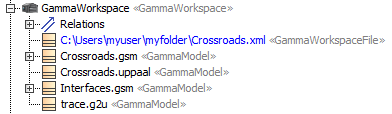
\includegraphics[width=10cm, keepaspectratio]{figures/contribution/gwsfinal.png}
	\caption{Workspace tartalma a transzformációk után}
	\label{fig:gwsfinal}
\end{figure}

Léteznek bizonyos felhasználási módok, hogy ezeket a modelleket MagicDraw-n kívül szeretnénk használni. A modelleket az \emph{Export models as .gcl...} akció végrehajtásával tudjuk kimenteni. Ezek a Gamma nyelvtanára fognak sorosodni.
A korábban bemutatott interfészek például ilyen formában fognak megjelenni:

\begin{lstlisting}
	package Interfaces
	interface LightCommands {
		out event displayNone
		out event displayRed
		out event displayGreen
		out event displayYellow
	}
	interface PoliceInterrupt {
		out event police
	}
	interface Control {
		out event toggle
	}
\end{lstlisting}

\subsection{Formális verifikáció}
 
A letranszformált modellek mellet meg kell tudni fogalmazni az ellenőrizendő feltételeket is. Ehhez előbb létre kell hozni egy \emph{Package}t a GammaWorkspaceben tetszőleges néven. Ebben tudunk létrehozni \emph{GammaCheckExpression}öket. Ezek fogják leírni az ellenőrizendő tulajdonságait a modellnek. Erre a Gamma Property nyelvtanát tudjuk használni. Tegyük fel, hogy elő szeretnénk írni, hogy a két \emph{TrafficLightCtrl} primary és secondary ne kerülhessenek egyszerre a "Green" állapotba. A kifejezést a \emph{GammaCheckExpression}  body mezőjébe meg kell megadni. Sajnos ennek a megadása kissé kényelmetlen, mert nincs \emph{content assist} sem semmilyen támogató funkció.

\begin{lstlisting}	
	E F [{state primary.NormalRegion.Green and state secondary.NormalRegion.Green}]
\end{lstlisting}

Az alábbi kifejezés azt írja le követelményként, hogy létezik-e út az állapottérben olyan állapotban, hogy mind két lámpa zöld. Ebben az esetben azt várjuk, hogy ez ne legyen igaz.

\newpage

\subsection{Eredmények kiértékelése és szimuláció}

A \emph{GammaCheckExpression}öket szintén a gyors menüben a  \emph{Gamma Transformation} alatt található \emph{Execute} paranccsal tudjuk futtatni. Az eredményt \aref{fig:verif1} ábrán láthatjuk.

\begin{figure}[!ht]
	\centering
	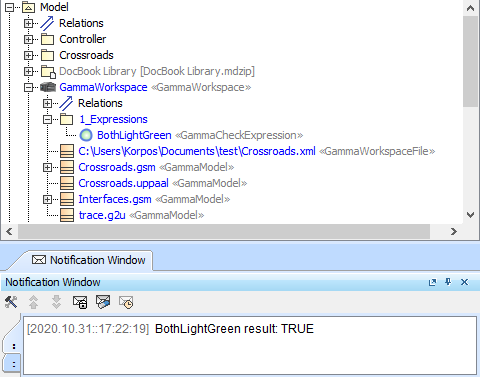
\includegraphics[width=10cm, keepaspectratio]{figures/contribution/verif1.png}
	\caption{Verifikáció futtatásának eredménye}
	\label{fig:verif1}
\end{figure}


Tehát a feltétel teljesül.

%TODO back-annotation, szimuláció

\subsection{Modell javítása}

A problémát úgy lehet kiküszöbölni talán a legkönnyebben, hogy a \emph{Controller}-be is felveszünk egy olyan állapotot amikor várakozik (\ref{fig:fixed} ábra).

\begin{figure}[!ht]
	\centering
	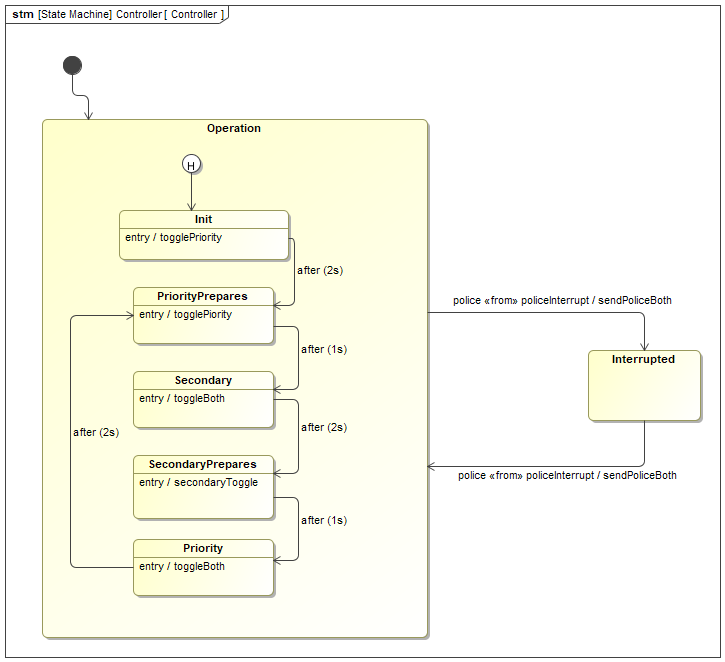
\includegraphics[width=10cm, keepaspectratio]{figures/contribution/ControllerFixed.png}
	\caption{Javított \emph{Controller} állapottérképe}
	\label{fig:fixed}
\end{figure}

A transzformációkat újra végre kell hajtani, hiszen a modell megváltozott. Viszont ha újra futtatjuk a verifikációt akkor már a tulajdonság nem lesz igaz, tehát valóban sikerült javítani a modellt (\ref{fig:verif2} ábra).

\begin{figure}[!ht]
	\centering
	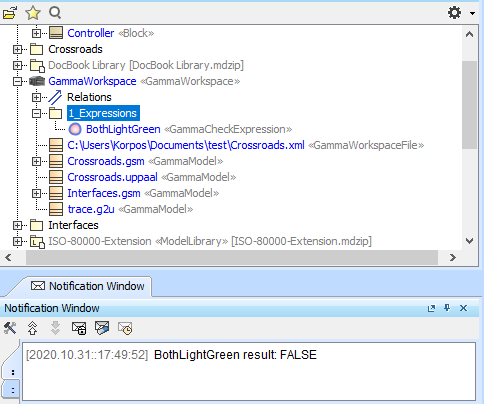
\includegraphics[width=10cm, keepaspectratio]{figures/contribution/verif2.png}
	\caption{Verifikáció futtatásának eredménye a javított modellen}
	\label{fig:verif2}
\end{figure}





\chapter{Értékelés}
\chapter{Összefoglalás}

Dolgozatomban a feladat kiírásnak megfelelően bemutattam az eszköz korábbi változatát, majd ismertettem azokat a módosításokat melyeket a szoftveren végeztem. A módosítások eredményeképp már kompozit, hierarchikus állapottérképek formális verifikációjára is lehetőség van, az ellenpéldák a modellben létrejönnek. A továbbfejlesztett eszköz működését bemutattam egy példán és mérésekkel vizsgáltam a beépülő modul teljesítményét.

\paragraph{A fontosabb kontribúciókéó:}
\begin{itemize}
	\item Komponensek transzformációja
		\begin{itemize}
			\item UML profil a komponens szemantika módosításához
			\item Támogatott modell struktúrák
			\item A transzformáció megvalósítása
			\item Validációs készlet tervezése
		\end{itemize}
	
	\item Példák, ellenpéldák megjelenítése
		\begin{itemize}
			\item UML profil a szemantika változtatásához
			\item Ellenpélda back-annotálása a SysML modellbe
			\item Szcenárió megjelenítésének vizsgálata különböző diagramtípusokon
			\item Kísérletek a szcenáriók végrehajtására a szimulátorral
		\end{itemize}
	\item Property nyelvtan felhasználása
		\begin{itemize}
			\item tulajdonságok definiálása a Gamma Property nyelvtanán speciális modell elemekben	
		\end{itemize}
	\item Megvalósítás értékelése teljesítmény szempontjából
		\begin{itemize}
			\item transzformáció végrehajtási idejének mérése
			\item a VIATRA minták memória igényének vizsgálata	
		\end{itemize}
\end{itemize}
A munkám eredményeként komponens és állapot alapú modelleken is végre lehet hajtani a formális verifikációt. A modellben back-annotáció formájában megjelennek a példák és ellenpéldák. A rendszer tulajdonságait pedig a Gamma \emph{Property} nyelvtanának segítségével lehet megfogalmazni.

\section{Lehetőségek az eszköz továbbfejlesztésére}

Az ellenpéldák megjelennek a modellben, de a szcenáriókat leíró diagramok automatikusan nem állnak elő. Ezek előállítása szintén segítené a mérnököket a modellek vizsgálatában. Ezen felül egy szimulátor motort is létre lehetne  hozni, ami lehetővé tenné az események helyes visszajátszását.

Ahogy arra a mérések is rámutattak van olyan megoldás aminek az alkalmazása teljesítmény problémához vezetett. Ezek kijavítása vagy más megoldásra cserélése a jövőben indokolt.





% Acknowledgements
%~~~~~~~~~~~~~~~~~~~~~~~~~~~~~~~~~~~~~~~~~~~~~~~~~~~~~~~~~~~~~~~~~~~~~~~~~~~~~~~~~~~~~~
%%----------------------------------------------------------------------------
\chapter*{\koszonetnyilvanitas}\addcontentsline{toc}{chapter}{\koszonetnyilvanitas}
%----------------------------------------------------------------------------

Szeretnék köszönetet mondani mindazoknak a feladat elvégzése során segítették a munkám: Farkas Rebekának, aki konzulensemként mindig segítőkész, pozitív hozzáállásával, és szakmai tanácsival, kritikáival segítette a dolgozat létrejöttét. Továbbá Molnár Vincének aki a Gamma Statechart Composition Framework használatát javasolta és ötleteket adott a megvalósítható funkciókra vonatkozóan. Köszönöm továbbá az IncQuery Labs-nak, hogy rendelkezésemre bocsátották a plug-in skeletonjukat, és a náluk töltött szakmai gyakorlatom során szerzett gyakorlati tapasztalatokat, amik jelentősen megkönnyítették az implementáció elkészítését.


% List of Figures, Tables
%~~~~~~~~~~~~~~~~~~~~~~~~~~~~~~~~~~~~~~~~~~~~~~~~~~~~~~~~~~~~~~~~~~~~~~~~~~~~~~~~~~~~~~
%\listoffigures\addcontentsline{toc}{chapter}{\listfigurename}
%\listoftables\addcontentsline{toc}{chapter}{\listtablename}


% Bibliography
%~~~~~~~~~~~~~~~~~~~~~~~~~~~~~~~~~~~~~~~~~~~~~~~~~~~~~~~~~~~~~~~~~~~~~~~~~~~~~~~~~~~~~~
\addcontentsline{toc}{chapter}{\bibname}
%\bibliography{bib/mybib}


% Appendix
%~~~~~~~~~~~~~~~~~~~~~~~~~~~~~~~~~~~~~~~~~~~~~~~~~~~~~~~~~~~~~~~~~~~~~~~~~~~~~~~~~~~~~~
%%----------------------------------------------------------------------------
\appendix
%----------------------------------------------------------------------------
\chapter*{\fuggelek}\addcontentsline{toc}{chapter}{\fuggelek}
\setcounter{chapter}{\appendixnumber}
%\setcounter{equation}{0} % a fofejezet-szamlalo az angol ABC 6. betuje (F) lesz
\numberwithin{equation}{section}
\numberwithin{figure}{section}
\numberwithin{lstlisting}{section}
%\numberwithin{tabular}{section}

%----------------------------------------------------------------------------
%\section{A TeXstudio felülete}
%----------------------------------------------------------------------------
%\begin{figure}[!ht]
%\centering
%\includegraphics[width=150mm, keepaspectratio]{figures/TeXstudio.png}
%\caption{A TeXstudio \LaTeX-szerkesztő.} 
%\end{figure}


%\label{page:last}
\end{document}
